%Made By Thomas Debelle
\documentclass{report}
\usepackage[a4paper, total={6in, 9in}]{geometry}
\usepackage[utf8]{inputenc}
\usepackage[french]{babel}
\usepackage{graphicx}
\usepackage{graphics}
\usepackage[T1]{fontenc}
\usepackage{amsmath}
\usepackage{hyperref}
\usepackage{amssymb}
\usepackage{listings}
\usepackage{wrapfig}
\usepackage{xcolor}
\usepackage{array}
\usepackage{float}
\usepackage{amsfonts}
\usepackage{fancyhdr}
\usepackage{titlesec}
\usepackage{xparse}


\definecolor{codegreen}{rgb}{0,0.6,0}
\definecolor{codegray}{rgb}{0.5,0.5,0.5}
\definecolor{codepurple}{rgb}{0.58,0,0.82}
\definecolor{backcolour}{rgb}{1.0,1.0,1.0}
\definecolor{codeblue}{rgb}{0,0,0.8}

\lstdefinestyle{mystyle}{
    backgroundcolor=\color{backcolour},   
    commentstyle=\color{codegray},
    keywordstyle=\color{codeblue},
    numberstyle=\tiny\color{codegray},
    stringstyle=\color{codeblue},
    basicstyle=\ttfamily\footnotesize,
    breakatwhitespace=false,         
    breaklines=true,                 
    captionpos=b,                    
    keepspaces=true,                 
    numbers=left,                    
    numbersep=5pt,                  
    showspaces=false,                
    showstringspaces=false,
    showtabs=false,                  
    tabsize=2,
    frame=shadowbox
}
\lstset{style=mystyle}
\lstset{language=Oz}

\hypersetup{
    colorlinks=true,
    linkcolor=black,
    filecolor=magenta,
    urlcolor=cyan,
    pdftitle={LINFO1104},
    pdfpagemode=FullScreen,
    }
\begin{document}


\begin{titlepage}
    \begin{figure}
        
\includegraphics[height = 2cm]{UCL_Logo.png}
        \label{fig:my_label}
    \end{figure}

    \hspace*{100cm}
    \centering
    \vspace*{7cm}

    {\Huge \textbf{Résumé de LINFO1104}}\\
    \vspace*{0.25cm}
    compilation du \today\\
    \vspace*{0.25cm}
    \Large{Thomas Debelle}\\

    \vspace*{9.5cm}
    {\Large Juin 2023}
\end{titlepage}


\tableofcontents
\newpage

\section*{Préface}

Bonjour à toi !\\

Cette synthèse recueille toutes les informations importantes données au cours, pendant les séances de tp et est amélioré grâce au note du Syllabus. Elle ne remplace pas le cours donc écoutez bien les conseils et potentielles astuces que les professeurs peuvent vous donner. Notre synthèse est plus une aide qui on l'espère vous sera à toutes et tous utiles.\\

Elle a été réalisée par toutes les personnes que tu vois mentionné. Si jamais cette synthèse a une faute, manque de précision, typo ou n'est pas à jour par rapport à la matière actuelle ou bien que tu veux simplement contribuer en y apportant ta connaissance ? Rien de plus simple ! Améliore la en te rendant \href{http://www.github.com/Tfloow/Q4_EPL}{ici} où tu trouveras toutes les infos pour mettre ce document à jour. (\textit{en plus tu auras ton nom en gros ici et sur la page du github})\\

Nous espérons que cette synthèse te sera utile d'une quelconque manière ! Bonne lecture et bonne étude.


\chapter{Introduction}
\section{Les Paradigmes}
Une paradigme, est une façon d'approcher et apporter une solution à un problème. De ce fait, chaque langage de programmation utilise 1 voir 2 paradigmes. Ce cours couvrira 5 paradigmes cruciaux qui sont:
\begin{enumerate}
\item "Functionnal Programming"
\item "Object Oriented Programming"
\item "Functional DataFlow Programming"
\item "Actor DataFlow Programming or Multi-Agent"
\item "Active Objects"
\end{enumerate}

Et pour découvrir ces paradigmes, nous utiliserons les langages de programmations "\href{https://fr.wikipedia.org/wiki/Oz_(langage)}{Oz}" qui est un langage de recherche multi paradigme ainsi que "\href{https://fr.wikipedia.org/wiki/Erlang_(langage)}{Erlang}" à la fin du cours.

\chapter{Les différents Paradigmes}
\section{Functional Programming}
Avec ce paradigme, on impose qu'une variable peut être nommé qu'une seule fois ! Donc: $X = 10$ mais on ne peut pas plus loin dire $X = 9$. $X$ est déjà attribué. On peut penser que cela risque d'être handicapant alors qu'en réalité, cela rend notre code plus simple à débuguer. De plus, nombreux sont les langages et microservices utilisés qui implémentent la programmation fonctionnelle.
Formellement, quand on déclare une variable et qu'on l'assigne à une valeur ceci se passe.
\begin{wrapfigure}{r}{.45\textwidth}
	\centering
    \includegraphics[width=.5\textwidth]{img/declVar.png}
    \caption{Déclaration d'une variable}
\end{wrapfigure}
Une chose importante à noter est que cette façon de programmer peut être réalisé dans n'importe quel langage de programmation. On peut également redéclarer un identificateur. C'est-à-dire écrire "$X = 42$" et plus loin en ayant redéclarer une variable "$X = 11$" car ces deux déclarations pointent à deux éléments totalement différents dans la mémoire et ont des \textit{scopes} différents.\\

Un "Scope" ou portée est une propriété centrale en programmation. En effet, c'est le scope qui nous permet d'avoir différente valeur pour des variables qui ont le même nom. Naturellement, elle ne représente pas la même chose car elle diffère de leur scope. On peut déterminer le scope d'une variable sans même exécuter le code. Il nous suffit d'analyser le code qui comprend un "\textcolor{red}{lexical scoping}" ou un "\textcolor{red}{static scoping}".
\begin{lstlisting}[escapechar=\%]
local
  X
in 
  X = 42 {Browse X}
  local X in
    X = 11 {Browse X}
  end
  {Browse X}
end
\end{lstlisting}


\chapter{Programmation symbolique}
\section{Listes}
On dit d'une liste est \textbf{récursive} si elle se définit par elle-même. C'est-à-dire elle fait appel à elle-même. On utilise la récursion pour les calculs et pour stocker des données.
Une liste est soit vide ou soit une pair \textit{d'une valeur suivi par une autre liste}.
\subsection{Définition formelle}
En utilisant la notation \textbf{Extended Backus-Naur Form} ou \textit{EBNF} pour les intimes, on écrit une liste comme: <List T> ::= nil | T '|' <List T>. Une chose importante à noter est le deuxième "ou" qui s'écrit comme '|' signifiant qu'il n'appartient pas à la définition de List T mais plutôt à l'ensemble T '|' <List T>. Si on lit ceci, on dirait "\textit{Une list d'élément représentant T correspond à un élément vide ou un élément représentant T suivi d'une autre Liste d'élément T}.\\

\begin{wrapfigure}{r}{.35\textwidth}
	\centering
	\includegraphics[width=.3\textwidth]{img/listTree.png}
\end{wrapfigure}
Donc une List d'entier se définit comme: <List <Int> >. Une chose importante à remarquer est que j'ai utilisé le mot "représentation" en effet <Int> n'est pas un entier mais une représentation d'entier.\\

Pour définir une liste en Oz, on utilise soit la notation \textcolor{blue}{[1 2 3]} ou \textcolor{blue}{1 | 2 | 3 | nil}.(il existe d'autre manière semblable qu'on verra plus loin) C'est 2 déclarations reviennent à la même chose en mémoire. Une utilité des listes est leur facilité à être représenté sous forme d'arbre comme montré ci-contre. La \textit{head} est accessible via \textcolor{blue}{list.1} et la \textit{tail} est obtenu via \textcolor{blue}{list.2}.

\section{Pattern matching}

Grâce à cette représentation en arbre, il est facile de voir si une liste est bien une liste.\\
Ci-contre, on voit une fonction classique en Oz qui analyse une liste et détermine si elle est d'une structure correcte. Le \textcolor{blue}{[]} correspond au cas où l'élément \textcolor{blue}{L} est une liste avec une Head et une Tail. On appelle cela une \textit{Clause} et H|T est le pattern de la clause. Le premier cas est définit par \textcolor{blue}{of}.
\begin{lstlisting}[escapechar=\%]
fun {Sum L}
  case L
  of nil then 0
  [] H|T then H+{Sum T}
  end
end
\end{lstlisting}
\newpage

\section{Introduction au langage Kernel}
Le langage Kernel est la première partie de la sémantique formelle d'un langage de programmation. Une règle importante est que tout programme écrit en programmation fonctionelle \textit{peut être traduit en langage kernel}.
Les grands principes du langage Kernel sont:
\begin{itemize}
	\item Tous les résultats intermédiaires de calculs sont visibles. Donc on a 1 opération par ligne et la déclaration en locale de toutes les variables.
	\item Toutes les fonctions deviennent des \textit{procédures anonymes} avec un argument en plus. Cet argument donne le résultat de la fonction.
	\item Les fonctions dans une fonction sont sortis de leur fonction et on leur donne un nouvel identificateur.
\end{itemize}
Les résultats de la traduction: Les programmes Kernel sont plus longs mais on voit facilement comment un programme s'exécute et on voit si il est \textit{tail-recursive}

\section{Les arbres}
Les arbres sont des structures de données extrêmement utiles et utilisées. On peut y stocker des données spécifiques, faire des calculs, ... Les arbres illustrent bien \textit{la programmation orienté but}. Par le standard \textit{EBNF}, on définit un arbre comme suit: <tree T> ::= leaf | t(T <tree T> ... <tree T>). Donc un arbre est une feuille ou \textit{leaf} qui est suivie par un ensemble de \textit{sous-arbres} (Il faut noter que le $t(...)$ est une façon d'écrire un \textit{record} de label "\textit{t}" qui est vu au \ref{record}). Les arbres sont forts similaires au liste si ce n'est que les listes n'ont qu'une sous-listes alors qu'un arbre peut avoir plusieurs sous-arbres.

\subsection{Ordered Binary tree}
Un arbre de ce type a 2 particularités:
\begin{itemize}
\item \textcolor{red}{Binary}: toutes les éléments hors les feuilles possèdes 2 sous-arbres.
\item \textcolor{red}{Ordered}: pour chaque arbre, la clé à gauche est plus petite que la clé de l'arbre et la clé à droite est plus grande.
\end{itemize}
Ce type d'arbre est très utile pour; par exemple, effectuer des recherches binaires et permet de facilement et rapidement trouver des données.

\subsubsection{Lookup K T}
Nous permet de trouver une valeur. Ce programme est plutôt simple et il nous suffit de regarder la clé de l'arbre où on est. Puis on compare avec notre recherche, si on est plus grand, on va à droite sinon à gauche. On répète le processus jusqu'à trouver la clé.\\
Lookup est très efficace car il s'exécute en \textcolor{red}{$log_2 n$}, le pire cas est si l'arbre n'est pas équilibré et il ressemble à une liste. Mais en général, en ayant un nombre suffisant de données, il est très rare d'avoir un arbre non équilibré.
\subsubsection{Insert K W T}
Il existe 4 possibilités.
\begin{enumerate}
\item remplace une feuille.
\item on remplace un noeud.
\item on remplace un sous-arbre à gauche.
\item on remplace un sous-arbre à droite.
\end{enumerate}
Le premier cas est le plus simple car on créé simplement un nouvel sous-arbre avec 2 feuilles. Si on remplace un noeud, on change la clé et la valeur du noeud.
Pour remplacer un sous-arbre, on garde les mêmes clés et valeur de Y pour le noeud mais on change le sous-arbre à gauche ou à droite en fonction.
\subsubsection{Delete K T}
Celle-ci est plus compliqué, on a 4 possibilités
\begin{enumerate}
\item La valeur qu'on veut supprimer n'existe pas
\item On supprime une feuille.
\item on supprime un sous-arbre à gauche.
\item on supprime un sous-arbre à droite.
\end{enumerate}
%\textcolor{red}{TODO} ajouter le code et l'explication

\section{Tuples et Records}

\subsection{Tuples}
Un tuple est une manière de stocker des données de différents tuples, l'\textit{ordre} est \textit{important} dans un tuple. On doit également donné un nom, un \textbf{label}.
\begin{lstlisting}
X = state(1 b 2)
{Browse {Label X}}
{Browse {Width X}}
\end{lstlisting}
La première ligne définit un tuple ayant pour \textit{label} "state". La seconde ligne imprime le label du tuple. La dernière affiche sa taille. (c'est donc un entier toujours positif ou $0$)\\
Les champs dans les tuples sont numérotés de\textbf{ $1$ à width $X$}. On appelle aussi le champ (field) une "\textit{feature}". Un tuple possède toutes ces features de manière consécutives.\\

On peut donc ainsi construire des structures de données plus compliqués comme des arbres:
\begin{lstlisting}
declare
Y = left(1 2) Z = right(3 4)
X = mid(Y Z)
\end{lstlisting}

\begin{figure}[H]
\centering
\includegraphics[width=5cm]{img/treeTuple.png}
\end{figure}
\subsubsection{Comparaison}
Il est très simple de comparer des tuples via "$==$", il faut simplement comparer leur value à chaque champ. Attention au \textit{loop} causé par les approches naïves.\\

\subsection{Similitude Tuples et liste}
En effet, une liste qui n'est autre que "H|T" peut facilement être traduit en tuple '|' (H T). Quand on peut déterminer un même élément via différentes manières, on appelle ça du \textit{sucre syntaxique}. Dans le \textit{kernel}, on fait au plus simple donc que des tuples.
\begin{lstlisting}[escapechar=\%]
List1 = [1 2 3]
List2 = (1:1 2:(1:2 2:(1:3 2:nil)))
List1 == List2 %//Vrai%
\end{lstlisting}

\subsection{Les Records} \label{record}
Les "\textit{records}" sont une \textbf{généralisation} des tuples. La différence avec les tuples est que le \textit{field} peut être n'importe quel valeur et ne doit pas être consécutif. Donc ceux-ci sont des \textit{records} corrects:
\begin{lstlisting}
X = state(a:1 2:a b:2)
Y = inv(3:a 2:b 1:c)
\end{lstlisting}
Donc la position d'une valeur et son \textit{field} n'importe plus et on peut déclarer dans le sens qu'on veut.\\
Si on ne nomme pas un \textit{field} dans un \textit{record}, Oz va attribuer un nombre commençant à $1$ et qui n'est pas utilisé par un autre champ.\\
\subsection{Résumé}
\begin{itemize}
\item Un \textit{atom} est un record de width $0$.
\item Un tuple est un record avec des champs étant numéroté de manière consécutive de $1$ à width $X$. (consécutive, donc on skip pas. pas forcément dans l'ordre dans la déclaration)
\item Une liste est réalisée avec des \textit{tuples} et des $(X \quad Y)$. $X$ étant une donnée et $Y$ étant une sous-liste de données.
\item $\textbf{1}$ seule \textit{structure de donné} dans le kernel pour rester simple.
\end{itemize}

\section{Sémantique Formelle}
\subsection{Les environnements}
Un environnement est une fonction qui passe des \textit{identifieurs} aux \textit{variables en mémoire} autrement dit: $E_1 = ({X \rightarrow x, Y \rightarrow y)}$

\subsubsection{Environnement contextuel}
Un \textit{environnement contextuel} d'une fonction contient tous les \textit{identificateurs} qui sont utilisés dans la fonction mais déclarés \textit{en dehors}. Donc ce sont des fonctions qui lorsqu'on appelle une variable va pointer en dehors du scope de la fonction.

\subsubsection{Stocker une Procédure}
Les procédures sont stocker dans la mémoire sous le forme de procédure anonyme symboliser par le "\$".
\begin{lstlisting}
local P Q in
  {Browse 'do something'}
  proc {Q}
    {P}
  end
  {Browse 'another something'}
end
\end{lstlisting}
Notre "proc {Q}" sera stocker comme: "q = (proc\{\$\}\{P\} end, \{$P\rightarrow p$\})". On lit donc, la procédure \textit{anonyme} (\$), fais un appel à P (\{P\}) et finit (end), son \textit{environnement contextuel} fait que lorsqu'on appelle "P" on va récupérer la valeur "p" en mémoire (\{$P\rightarrow p$\}). Donc on voit que l'\textit{environnement contextuel} est stocké avec le code de procédure.\\
On appelle également la valeur d'une procédure une "\textit{closure}" ou une "\textit{lexically scoped closure}" car elle ferme les identificateurs libres quand définis.\\
Donc l'avantage d'un environnement contextuel est d'être sûr qu'on appellera la bonne valeur même si elle est déclaré en dehors de la fonction.\\

Un \textit{identificateur libre} est un identificateur utilisé dans une \textit{fonction} qui est déclaré \textit{en dehors} de la fonction.\\
Les arguments d'une procédure \textbf{ne sont pas} des identificateurs libres car l'argument défini l'identificateur.

\subsection{Sémantique}
Il est important de comprendre le fonctionnement même d'un programme car si on ne comprend pas comment celui-ci fonctionne, il nous domine. \textit{If you do not understand something, then you do not master it – it masters you!}
\subsubsection{Définition}
La \textit{sémantique} d'un langage de programmation est une explication \textit{précise} de comment un programme s'exécute. Nous verrons la sémantique pour tous les paradigmes. Il en existe 4 types:
\begin{enumerate}
\item \textcolor{red}{Sémantique opérationnelle}: explique un programme sur base d'\textit{exécution} sur un PC simplifié appelé \textit{la machine abstraite}. $\rightarrow$ Fonctionne pour tous les paradigmes.
\item \textcolor{red}{Sémantique axiomatique}: explique un programme sur base d'\textit{implication}. C'est-à-dire que certaines \textit{propriétés} présentes avant l'exécution, et d'autres seront présentes après. $\rightarrow$ très utilisé pour la programmation orientée objet comme \textit{Java}.
\item \textcolor{red}{Sémantique de notation}: explique un programme comme une \textit{fonction} sur un domaine abstrait. Donc simplifie l'analyse mathématique d'un programme. (utilisé dans \textit{Haskell} et \textit{Scheme})
\item \textcolor{red}{Sémantique logique}: explique un programme comme étant un \textit{modèle logique} basé sur des \textit{axiomes logiques}. Le résultat est une propriété correcte dérivée des axiomes. (cela est implémenté par exemple dans \textit{Prologue} ou dans la \textit{programmation sous contrainte})
\end{enumerate}

\subsection{Sémantique opérationnelle}
Ce type de sémantique à 2 parties majeures:
\begin{itemize}
\item \textcolor{red}{Langage Kernel}: traduit le programme en langage Kernel.
\item \textcolor{red}{Machine abstraite}: puis exécute le programme sur la machine abstraite.
\end{itemize}

\subsubsection{1. Langage Kernel complet}
Pour définir correctement une sémantique, il faut tout d'abord s'intéresser à son langage Kernel complet. On peut également prouver qu'un programme est correct en analysant son kernel. Par exemple, prenons ce code kernel:
\begin{lstlisting}[escapechar=\%]
<s> ::= skip 
  | %$<s>_1 <s>_2$% 
  | local <x> in <s> end 
  | %$<x>_1=<x>_2$% 
  | <x>=<v> 
  | if <x> then %$<s>_1$% else %$<s>_2$% end 
  | {<x> %$<y>_1,...,<y>_n$%} 
  | case <x> of <p> then %$<s>_1$% else %$<s>_2$% end

<v> ::= <number> | <procedure> | <record>  
<number> ::= <int> | <float> 
<procedure> ::= proc {$ %$<x>_1, ..., <x>_n$%} <s> end
<record>, <p> ::= <lit> | <lit>(%$<f>_1:<x>_1, ..., <f>_n:<x>_n$%)
\end{lstlisting}
donc "<s>" contient le programme exécuté, "<v>" est une structure de donné contenant différent type de structure de donné qui sont définis juste en dessous. 

\subsubsection{2. La machine abstraite}
Voici ci-dessous comment s'exécute un programme initialement.

\begin{minipage}[t]{0.45\linewidth}
\begin{lstlisting}[caption={Programme en Oz}]
local X in
  local B in
    B=true
    if B then X=1 
    else skip end
  end
end
  
\end{lstlisting}
\end{minipage}
%
\begin{minipage}[t]{0.45\linewidth}
\begin{lstlisting}[caption={État initial}]
([(local X in 
     local B in 
       B=true
       if B then x=1 else skip end
     end
   end, {})],
 {})
\end{lstlisting}
\end{minipage}

Au début, l'environnement et la mémoire sont vides. L'état d'exécution est écrit typiquement comme:
\begin{lstlisting}[escapechar=\%]
([(<s>,E)], %$\sigma$)
\end{lstlisting} %trouver comment utiliser un code dans lst
Sur la machine abstraite, on va d'instructions en instructions. C'est-à-dire on descend petit à petit.
donc on a pour la suite:

\begin{minipage}[t]{0.45\linewidth}
\begin{lstlisting}[caption={On avance d'un cran}, escapechar=\%]
([(local B in
     B=true
     if B then X=1 else skip end
   end, {X %$\rightarrow$% x})]),
 {x})
\end{lstlisting}
\end{minipage}
%
\begin{minipage}[t]{0.45\linewidth}
\begin{lstlisting}[caption={On avance d'un cran}, escapechar=\%]
([((B=true
    if B then X=1 else skip end),
 {B %$\rightarrow$% b, X %$\rightarrow$% x})]),
 
 {b, x})
\end{lstlisting}
\end{minipage}

On voit que au fur et à mesure qu'on descend, la pile de mémoire et d'environnement s'agrandit. Ensuite on va \textit{séparer} la \textit{composition séquentielle} comme suit:

Une nouvelle instruction va s'ajouter à cause du "then" de notre condition:

\begin{minipage}[t]{0.45\linewidth}
\begin{lstlisting}[caption={On avance d'un cran}, escapechar=\%]
([(X=1, {B %$\rightarrow$% b, X %$\rightarrow$% x})],
 {b=true, x})
\end{lstlisting}
\end{minipage}
%
\begin{minipage}[t]{0.45\linewidth}
\begin{lstlisting}[caption={On avance d'un cran}, escapechar=\%]
([],
 {b=true, x=1})
\end{lstlisting}
\end{minipage}

\subsubsection{3. Définir la machine abstraite}
\begin{itemize}
\item Pour chaque instructions dans le langage Kernel, on associe sa règle dans la machine abstraite
\item Chaque instructions prends un état d'exécution en entrée et sort un état d'exécution en sortie $\rightarrow (ST, \sigma)$.
\end{itemize}
L'instruction la plus simple est "\textcolor{blue}{skip}" car il fonctionne comme $([(skip, E), S_2, ..., S_n], \sigma)$ et renvoie $([S_2,..., S_n], \sigma)$ 

\begin{center}
\begin{tabular}{|c|c|c|}
\hline
Instructions & entrée & sortie\\
\hline
\textcolor{blue}{skip} & $1$ & $2$\\
\hline 
\textcolor{blue}{$(<s>_1 <s>_2)$} & $([(S_a S_b), S_2, ..., S_n], \sigma)$ & $([S_a, S_b, S_2, ..., S_n], \sigma)$\\
\hline 
\textcolor{blue}{local in <x> in <s> end} & $([(\text{local } <x> \text{ in } <s> \text{ end }, E)$ & $([(<s>, E+\{<x>\rightarrow x\})$\\
 & $, S_2, ..., S_n], \sigma)$ & $, S_2, ..., S_n], \sigma)$\\
\hline 
\end{tabular}
\end{center}
Il y a également d'autres types d'instructions dont on détaillera pas le langage en machine abstraite:

\begin{itemize}
\item \textcolor{blue}{<x>=<v> (crée et assigne une valeur)}: quand <v> est une procédure, on \textbf{doit} créer un environnement contextuel.
\item \textcolor{blue}{if <x> then $<s>_1$ else $<s>_2$ end (condition)} : si <x> n'est pas attribué, l'instruction va attendre (“\textit{block}”) jusqu'à ce que <x> soit attribuer à une valeur.
\item \textcolor{blue}{case <x> of <p> then $<s>_1$ else $<s>_2$ end} : Le system de "\textit{case}" se construit en combinant des structures de données Kernel.
\item \textcolor{blue}{\{$<x> <y>_1, ..., <y>_n$\}} : ceci est la base de l'abstraction de donnée
\end{itemize}
Par ailleurs, voici d'autres concepts de machine abstraite:
\begin{itemize}
\item \textcolor{blue}{Single-assignment memory }\textcolor{red}{$s = \{x_1=10, x_2, x_3=20\}$}: Définition d'une variable et la valeur associée.
\item \textcolor{blue}{Environnement }\textcolor{red}{$E = \{X \rightarrow x, Y \rightarrow y\}$}: Lien entre un identificateur et son lien dans la mémoire
\item \textcolor{blue}{Instruction sémantique }\textcolor{red}{$(<s>, E)$}: Une instruction avec son environnement.
\item \textcolor{blue}{Stack Sémantique }\textcolor{red}{$ST = [(<s>_1,E_1), ..., (<s>_n,E_n)]$}: Un stack d'instructions sémantiques.
\item \textcolor{blue}{État d'exécution }\textcolor{red}{$(ST,\sigma)$}: Une paire d'un stack sémantique et sa mémoire.
\item \textcolor{blue}{Execution }\textcolor{red}{$(ST_1,s_1) \rightarrow (ST_2,s_2) \rightarrow (ST_3,s_3) \rightarrow ...$}: Une séquence d'état d'exécution. 
\end{itemize}

\subsubsection{4. Programme correct}
grâce à la sémantique, on sait prouver qu'un programme est correct. On dit qu'un programme produit une solution correcte, on l'appelle une \textit{spécification}.\\
Donc on prouve qu'un programme satisfait la \textit{spécification} quand on utilise une certaine \textit{sémantique}. La sémantique lie le \textit{programme} à un résultat mathématique appelé \textit{spécification}.\\

Donc on lie une vérité mathématique à un programme. Et on prouve cela via ces différentes étaps: (exemple avec une factorielle)

\begin{enumerate}
\item On commence avec la spécification du programme.
\item Notre programme est \textit{récursif} donc on va utiliser une preuve mathématique par \textit{induction}.
\item On doit prouver le cas de base et le cas général.
\item On utilise la sémantique pour prouver la véracité de notre programme.
\end{enumerate}

\subsubsection{5. Procédures}
Les procédures sont la base de toutes \textcolor{red}{abstractions de données}.\\
Il y a deux choses importantes dans une \textit{procédure}: sa \textcolor{red}{définition} et son \textcolor{red}{appel}.\\

\textcolor{red}{Définition}: on crée l'environnement \textit{contextuel}. Puis, on stocke le code de la procédure et son environnement.\\

\textcolor{red}{Appel}: on crée un nouvel environnement combinant l'environnement \textit{contextuel} de la procédure et les variables \textit{formelles}. Ensuite, le tout est exécuté.
\begin{lstlisting}
local Z in 
  Z=1
  proc{P X Y}Y=X+Z end
end
\end{lstlisting}
Ici, le seul identificateur \textit{libre} est \textbf{Z} qui est donc déclaré en dehors de la \textit{procédure}. Donc à l'exécution de \textbf{P}, \textbf{Z} est connu donc \textbf{Z} fait partie de l'environnement contextuel de la \textit{procédure}.
\begin{lstlisting}
local P in
  local Z in 
    Z=1
    proc{P X Y}Y=X+Z end
  end
  local A B in
     A=10
    {P A B}
    {Browse B}
  end
end 
\end{lstlisting}
Ici, à la ligne de la création de la procédure P, son environnement contextuel est $E_c = \{Z \rightarrow z\}$.On va stocker dans la mémoire notre instruction et son environnement \textit{contextuel} c'est la \textit{semantic rule}. Au moment de l'exécution de P avec les valeurs A et B, on va donc ajouter un environnement qui est de la sorte: $E_P = \{Y \rightarrow b, X \rightarrow a, Z \rightarrow z\}$. Donc ce deuxième environnement est stocker dans le \textit{stack sémantique} \textbf{pas} dans la mémoire avec le fonction !
Donc en langage \textit{sémantique}, la définition d'une procédure ressemble à cela:
\begin{itemize}
\item \textbf{Instruction sémantique}: (<x>=\textcolor{blue}{proc}\{\$ $<x>_1, ..., <x>_n$\} <s> \textcolor{blue}{end}, E)
\begin{itemize}
\item \textbf{Arguments formels}: $<x>_1, ..., <x>_n$
\item \textbf{Identificateurs libres de <s>}: $<z>_1, ..., <z>_k$
\item \textbf{Environnement contextuel}: $E_C = E_{|<z>_1, ...n <z>_k}$ (que les identificateurs libres)
\end{itemize}
\item Cela crée une liaison en mémoire de la forme: x(\textcolor{blue}{proc}$\{\$<x>_1, ..., <x>_n\}$<s>, \textcolor{blue}{end}, $E_C$)
\end{itemize}
Maintenant, voyons pour un \textit{appel sémantique}:
\begin{itemize}
\item \textbf{Instruction sémantique}: (\{$\langle x \rangle \langle y \rangle_1 ... \langle y \rangle_n$\}, E)
\begin{itemize}
\item Si la condition est \textit{false} donc $E(\langle x \rangle)$ n'est pas lié.
\item Si $E(\langle x \rangle)$ n'est \textbf{pas} une procédure, on a une erreur de \textit{condition}.
\item Si $E(\langle x \rangle)$ est une procédure \textit{mais} avec le mauvais nombre d'argument, on a aussi une erreur de \textit{condition}.
\end{itemize}
\end{itemize}
Une chose primordiale à comprendre est comment sont stocké les instructions. Elles sont stocké sur une \textbf{pile} (\textit{stack}). Donc on a l'instruction sémantique sur le stack: (\{$\langle x \rangle \langle y \rangle_1 ... \langle y \rangle_n$\}, E) avec la définition de procédure dans la \textit{mémoire} comme cela: $E(\langle x \rangle) = proc\{\$ \langle z \rangle_1, ..., \langle z \rangle_n\} \langle s \rangle \text{end}, E_c)$ \\
Ensuite, on met ces instructions sur la \textit{pile} $(\langle s \rangle , E_C + \{\langle z \rangle_1 \rightarrow E(\langle y \rangle_1), ..., \langle z \rangle_n \rightarrow E(\langle y \rangle_n)\})$\\

La machine abstraite fait 2 choses:
\begin{enumerate}
\item \textcolor{red}{Adjonction}: $E_2 = E_1+\{X \rightarrow y\}$ Donc ajoute une paire (identificateur $\rightarrow$ variable) à l'environnement. Ré-écrit par dessus $E_1$ si existe déjà. Utile pour \textcolor{blue}{local} $<x>$ \textcolor{blue}{in} $<s>$ \textcolor{blue}{end}.
\item \textcolor{red}{Restriction}: $E_C = E_{|\{X,Y,Z\}}$ Donc limite les \textit{identificateurs} dans un environnement. On a besoin de cela pour calculer l'environnement \textit{contextuel}.
\end{enumerate}
Une adjonction:
\begin{lstlisting}[escapechar=\%]
local X in
  (E1) X=1 
  local X in 
    (E2) X=2 
    {Browse X}
  end 
end
E1 = {Browse %$\rightarrow$% b, X %$\rightarrow$% x}
E2 = E1 + {X %$\rightarrow$% y} = {Browse %$\rightarrow$% b, X %$\rightarrow$% y}
\end{lstlisting}
Une restriction:
\begin{lstlisting}[escapechar=\%]
local A B C AddB in
  A=1 B=2 C=3 %\textcolor{red}{(E)}%
  fun {AddB X} %\textcolor{red}{(EC: contextual environment)}%
    X+B
  end
end
E = {A %$\rightarrow$% a, B %$\rightarrow$% b, C %$\rightarrow$% c, AddB %$\rightarrow$% a' }
%$E_C$% = %$E_{|\{B\}}$% = {B %$\rightarrow$% b }
\end{lstlisting}
\subsection{Résumé}
Définir la sémantique permet de relier les programmes au mathématique. On donne des instructions \textit{sémantique} au \textit{kernel} pour qu'il sache comment exécuter dans la \textit{machine abstraite}. La sémantique nous permet de prouver qu'un programme est \textit{correct}.\\
La sémantique est au cœur de la programmation. Une nouvelle librairie est comme si on ajoutait des instructions au programme donc on augmente sa sémantique.\\
Quand on écrit un programme, il faut comprendre la sémantique (l'utilisateur n'a pas besoin de savoir). La sémantique doit être simple et complète.\\
On peut voir la sémantique comme le langage de programmation \textit{ultime}.\\
Il ne faut pas oublier que les pc sont baser sur les mathématiques \textit{discrètes}.

\section{Rappel procédure sémantique}
Tout d'abord, en programmation nous avons différentes étapes qui reposent chacun sur les précédentes. Fermeture $\rightarrow$ Programmation d'ordre supérieur $\rightarrow$ Abstraction des données $\rightarrow$ Technologie de l'information.\\

Rappel sur l'exécution d'un programme:
\begin{lstlisting}[escapechar=\%]
{Browse {Inc 10}}		#Langage pratique (classique)
%\hrulefill%
local M in		 	#Langage Kernel
  local N in
    M=10
    {Inc M N}
    {Browse N}
  end
end
\end{lstlisting}
A l'exécution,$[(\{Inc M N\},\{M\rightarrow m,N \rightarrow n,Inc \rightarrow i,Browse \rightarrow b\}), (\{Browse N\},\{M \rightarrow m,N \rightarrow n,Inc \rightarrow i,Browse \rightarrow b\})],
\{m=10,n,i=(proc \{\$ X Y\} Y=X+A end, \{A \rightarrow a\}), a=1,b=(... browser code…)\}$ et Inc va référencer cela:\\
$[(Y=X+A,\{A\rightarrow a,X \rightarrow m,Y \rightarrow n\}), (\{Browse N\},\{M \rightarrow m,N \rightarrow n,Inc \rightarrow i,Browse \rightarrow b\})],
\sigma$\\
Il est important de remarquer que dans la mémoire, quand on stocke une procédure, on stocke le tout donc avec son environnement contextuel.


\chapter{Programmation d'ordre supérieur}
Ce concept découle directement du concept d'\textit{environnement contextuel}. Dans un \textit{procédure} ou \textit{fonction} (les mêmes pour un langage kernel) peuvent prendre des valeurs ou des fonctions en arguments.
\subsubsection{Définition}
\begin{itemize}
\item Une fonction est dit \textcolor{red}{de premier ordre} si elle ne prend et ne ressort aucune fonction.
\item Une fonction est \textcolor{red}{N+1} si son entrée et sortie prennent en tout $N$ fonctions en argument.
\end{itemize}
Nomenclature des différentes fonctions:
\begin{itemize}
\item \textbf{Une génératrice} est le fait de prendre une fonction en entrée d'une fonction.
\item \textbf{Une instantiation} est le fait de retourner une fonction en sortie d'une fonction.
\item \textbf{Une composition de fonctions} est le fait de prendre 2 fonctions en entrée et on retourne leur composition.
\end{itemize}

\subsubsection{Utilisation}
Via la programmation d'ordre supérieure, on peut cacher un accumulateur. On dit qu'on fait une \textit{abstraction d'accumulateur}.\\
Une fonction type est la fonction \textbf{FoldL} (\textit{reduce}). En effet, la fonction FoldL fait:
\begin{lstlisting}
declare
fun {FoldL L F U}
  case L
  of nil then U
  [] H|T then {FoldL T F {F U H}}
  end
end

{FoldL LIST Function Acc}
\end{lstlisting}
On peut, un peu dans le même style, faire de l'encapsulation afin de cacher sa valeur à l'intérieur. $\rightarrow$ C'est la base de \textit{l'abstraction de donnés}.\\

Il faut faire attention à l'\textbf{exécution retardé}. En effet, si on ne stocke pas le résultat d'une fonction, elle ne sera exécuté que quand on appellera la valeur. Donc cela peut prendre beaucoup de place en mémoire de stocker une fonction plutôt que son résultat.

%Here

\chapter{Lambda Calcul}
\begin{enumerate}
\item C'est un modèle de calcul qui est \textcolor{red}{Turing complete}. 
\item \textbf{Tous} les types de données peuvent être encodé en lambda calcul.
\item Par le théorème de \textbf{Church-Rosser}, le lambda calcul est \textcolor{red}{confluent}. Même résultat peu importe l'ordre de réduction
\item C'est la base de la programmation ordre supérieur et de la programmation formelle.
\end{enumerate}
\section{Introduction}
Le \textit{lambda calcul} est une manière mathématique formelle pour représenter des calculs informatiques. Cela a été créé avant l'arrivée des ordinateurs. Cela ne contient que des \textbf{définitions}, \textbf{appels} et utilise des \textbf{liens de variables} et de la \textbf{substitution}.\\

Le \textit{lambda calcul} est une manière universelle de calcul. On peut l'utiliser pour simuler des \textbf{machines de Turing}.

\subsection{Fonctionnement}
Le lambda calcul n'a que des \textit{fonctions anonymes d'un seul argument}. Donc si on veut en avoir plusieurs, il faut combiner les fonctions:
\begin{lstlisting}[escapechar=\%]
sum_square(x,y) = %$x^2+y^2$ //fonction classique%
(x,y) %$\rightarrow x^2 + y^2$ //fonction anonyme%
x %$\rightarrow$% (y %$\rightarrow x^2 + y^2$%) %//d'une seul argument%
%$\lambda x. \lambda y. x^2+y^2$ //en lambda calcul%    
\end{lstlisting}
Le fait de combiner et de "\textit{nest}" des fonctions s'appellent le \textcolor{red}{currying}.

\subsection{Syntaxe}
Les expressions lambdas sont composées de:
\begin{itemize}
\item Variables (x,y, ...)
\item Du symboles d'abstractions ($\lambda$) et de point (.)
\item Et des parenthèses
\end{itemize}
En syntaxe EBNF c'est:
\begin{lstlisting}[escapechar=\%]
t ::= x | (%$\lambda$%x.t) | %$t_1 \quad t_2$%
\end{lstlisting}
($\lambda$x.t): est appelé une abstraction (\textit{définition de fonction})\\
$t_1 \quad t_2$: c'est \textit{l'appel de fonction}.

\subsection{En Oz}
\begin{enumerate}
\item La définition de fonction ($\lambda$x.t)
\begin{lstlisting}[escapechar=\%]
fun %\{\$ X\}% T end
\end{lstlisting}
\item L'appel de fonction ($t_1 \quad t_2$)
\begin{lstlisting}[escapechar=\%]
%\{$T_1 \quad T_2$\}%
\end{lstlisting}
\end{enumerate}
Le currying en Oz:
\begin{enumerate}
\item Définition
\begin{lstlisting}[escapechar=\%]
F = fun %\{\$ X\}% fun %\{\$ Y\}% T end end
\end{lstlisting}
\item Appel
\begin{lstlisting}[escapechar=\%]
%\{\{F X\} Y\}%
\end{lstlisting}
\end{enumerate}

\subsection{Sémantique des expressions lambdas}
Le sens d'une expression lambda dépend de comment on peut la réduire. Il en existe 3 types.
\begin{enumerate}
\item \textcolor{red}{$\alpha$-renaming}: change le nom des variables liés
\item \textcolor{red}{$\beta$-reduction}: applique une fonction à un argument
\item \textcolor{red}{$\eta$-reduction}: enlève les variables inutilisés
\end{enumerate}

\subsubsection{Variables libres et liées}	
Si nous avons: $\lambda x.t$ on dit que \textit{l'opérateur} $\lambda x$ lie la variable $x$ à $t$. Mais la variable $t$ est libre car n'est lié à \textit{aucune} fonction. Si $x$ est libre dans $t$ alors on dit qu'on \textcolor{blue}{capture} $x$.\\
On dénote $FV(t)$ l'ensemble des variables libres:
\begin{itemize}
\item $FV(x) = \{x\}$ où $x$ est une variable
\item $FV(\lambda x.t) = FV(t) \textbackslash \{x\}$
\item $FV((t_1 \quad t_2))=FV(t_1) \cup FV(t_2)$
\end{itemize}

\subsubsection{$\alpha$-renaming}
Ainsi, on peut changer le nom d'une variable lié:
\begin{lstlisting}[escapechar=\%]
%$\lambda$% x. x %$\rightarrow_{\alpha}\lambda$%y. y
\end{lstlisting}
Il faut faire attention à ce qu'on ait pas de \textit{conflit de nom} et de \textit{capture de variable}.\\
Des termes qui diffèrent d'un $\alpha$-renaming sont dits $\alpha$-équivalents.

\subsubsection{Substitution} \label{sub}
La substitution de $t_1[x:=t_2]$ remplace toutes les occurrences libres de x dans $t_1$ par $t_2$.\\
On a parfois recourt à l'$\alpha$-\textit{renaming}. En effet, la substitution ne peut pas \textit{capturer} des variables libres. Donc $(\lambda x.y)[y:=x]$ peut être transformé en $(\lambda z.y)[y:=x]$. La définition:
\begin{align*}
x[x:=t] &= t & y[x:=t]&=y, \text{ if } x \neq y & (t_1 \quad t_2)[x:=t]&= (t_1[x:=t])(t_2[x:=t])\\
(\lambda x.t_1)[x:=t_2]&= \lambda x.t_1 & (\lambda y.t_1)[x:=t_2]&= \lambda y.(t_1[x:=t_2]),& \text{ if } x &\neq y \wedge y \notin FV(t_2)
\end{align*}


\subsubsection{$\beta$-reduction}
C'est une application de fonction et se décrit via la substitution. (cfr \ref{sub})\\
Définition:  $(\lambda x.t_1) t_2 \rightarrow t_1[::=t_2]$\\
Exemple: $(\lambda x.(x \quad x))y \rightarrow (y \quad y)$

\subsubsection{$\eta$-reduction}
C'est l'idée que 2 fonctions sont les \textit{mêmes} si elles produisent le \textit{même résultat} pour tous les arguments possibles. On appelle cela \textcolor{red}{extensibilité}. Donc 2 fonctions sont les mêmes si elles ont les mêmes propriétés extérieures.\\
Définition: $\lambda x.(t \quad x) \rightarrow t$ if $x \notin FV(t)$

\begin{figure}[H]
\centering
\includegraphics[width=6cm]{img/lambdaCal.png}
\caption{Résumé}
\end{figure}

\subsubsection{Convention de notation}
Quand on manipule des expression lambda, il est important de suivre quelques règles:
\begin{itemize}
\item Enlever les parenthèses les plus extérieur. ex: $(t_1 \quad t_2) \rightarrow t_1 \quad t_2$
\item Les applications sont associatives depuis la gauche. ex: $t_1 \quad t_2 \quad t_3 \rightarrow ((t_1 \quad t_2) \quad t_3)$
\item On étend vers la droite ex: $\lambda x.t_1 t_2 \rightarrow \lambda x.(t_1 t_2)$
\item On peut simplifier les séquences d'abstractions. ex: $\lambda x. \lambda y. \lambda z.t \rightarrow \lambda xyz.t$
\end{itemize}

\section{Types de données}
Le lambda calcul peut faire tout type de calcul, il est \textcolor{red}{Turing complete}.\\
Pour le démontrer, on va encoder des chiffres, opérations, ... en lambda calcul. Donc tous les chiffres, booléens, ... seront encodés en lambda calcul

\subsection{Nombres}
On utilise une notation appelée \textcolor{red}{Church Numerals}:
\begin{itemize}
\item $0 \triangleq \lambda f.(\lambda x.x)$
\item $1 \triangleq \lambda f.(\lambda x.(f \quad x))$
\item $2 \triangleq \lambda f.(\lambda x.(f (f \quad x))$
\item $3 \triangleq \lambda f.(\lambda x.(f (f (f \quad x))$
\end{itemize}
On peut remarquer que ces fonctions sont d'ordre supérieur. En effet, elles prennent en argument une fonction et ressortent une fonction. (d'un seul argument)\\
Le nombre $n$ retourne donc la fonction qui est une composition de $n$ fois de f. Donc on dit que \textbf{f est appliqué n fois}.

\subsection{Opérations}
\subsubsection{Fonction successeur}
Prend le nombre de Church $n$ et retourne $n+1$.
\begin{align*}
SUCC &\triangleq \lambda n.\lambda f.\lambda x.f((n \quad f)x) & SUCC &\triangleq \lambda n.\lambda f.\lambda x.f(n \quad f \quad x)
\end{align*}

\subsubsection{Addition}
Retourne donc la composition de $m+n$.
\begin{align*}
PLUS &\triangleq \lambda m.\lambda n.\lambda f	. \lambda x.(m \quad f)((n \quad f)x) & PLUS &\triangleq \lambda m.\lambda n.\lambda f	. \lambda x.m \quad f(n \quad f \quad x)
\end{align*}

\subsubsection{Multiplication}
\begin{align*}
MULT &\triangleq \lambda m.\lambda n.\lambda f.m (n \quad f) & MULT &\triangleq \lambda m.\lambda n.m (PLUS \quad n)\quad 0
\end{align*}
La deuxième façon de faire $MULT$ est comme si on disait, "fait une somme m fois en commençant à 0.

\subsubsection{Exponentielle}
\begin{align*}
POW &\triangleq \lambda b.\lambda e.e \quad b
\end{align*}

\subsubsection{Prédécesseur}
\begin{align*}
PRED &\triangleq \lambda n.\lambda f.\lambda x.n (\lambda g.\lambda h.h (g f)) (\lambda u.u)
\end{align*}

\subsubsection{Soustraction}
Grâce à la méthode du prédécesseur, on peut définir la soustraction:
\begin{align*}
SUB \triangleq \lambda m.\lambda n.n \quad PRED \quad m
\end{align*}
Donc pour $m-n$ on effectue la fonction prédécesseur $n$ fois en commençant à $m$. 

\subsection{Opération logique}

\subsubsection{Booléens}
\begin{align*}
TRUE &\triangleq \lambda x.\lambda y.x & FALSE &\triangleq \lambda x.\lambda y.y
\end{align*}

\subsubsection{Opérateur logique}
\begin{align*}
AND &\triangleq \lambda p.\lambda q.p \quad q \quad p & OR &\triangleq \lambda p.\lambda q.p \quad p \quad q\\
NOT &\triangleq \lambda p.p \quad FALSE \quad TRUE & IFTHENELSE &\triangleq \lambda p.\lambda a.\lambda b.p \quad a \quad b
\end{align*} 

\subsubsection{Prédicat}
Ce sont des fonctions qui retournent une valeur booléenne:
\begin{align*}
ISZERO &\triangleq \lambda n.n (\lambda x.FALSE) TRUE & LEQ &\triangleq \lambda m.\lambda n.ISZERO (SUB \quad m \quad n)
\end{align*}

\subsubsection{Paire}
Ce sont des tuples de \textit{width = 2} et peuvent être définis en terme de booléens:
\begin{align*}
PAIR &= (x,y) \text{ le tuple} & PAIR &\triangleq \lambda x.\lambda y.\lambda f.f \quad x \quad y\\
FIRST &\triangleq \lambda p.p \quad TRUE & SECOND &\triangleq \lambda p.p \quad FALSE\\ 
NIL &\triangleq \lambda x.TRUE & NULL &\triangleq \lambda p.p (\lambda x.\lambda y.FALSE)
\end{align*}
Ceci nous introduit à l'abstraction de donnée. Une chose cruciale à comprendre est que depuis les 3 principes simples du lambda calcul, (définition de fonction, utilisation de fonction, des variables en arguments) on peut tout réaliser !

\subsubsection{Liste}
En sachant qu'une liste est un ensemble de valeur de nil, on sait utiliser des listes en lambda calcul. On peut même les utiliser pour "\textit{simplement}" définir la fonction PRED via SHIFTINC:
\begin{align*}
SHIFTINC &\triangleq \lambda x.PAIR (SECOND \quad x) (SUCC (SECOND \quad x)) \quad (m,n) \rightarrow (n,n+1)\\
PRED &\triangleq \lambda n.FIRST (n \quad SHIFTINC (PAIR \quad 0 \quad 0))
\end{align*}
En effet cela fonctionne car le premier élément sera $n-1$ par rapport au second.

\subsection{Fonctions récursives}
Comme les fonctions sont anonymes, on ne peut pas faire d'appel direct récursif. On va faire en sorte qu'une fonction devient l'argument d'une expression lambda. Par exemple:
$G \triangleq \lambda f.\lambda n.$(if n = 0 then 1 else n(f n-1))

\subsubsection{Y combinator}
Cela nous permet de passer de $Y(g)$ à $g(Y \quad g)$. Ainsi, on sait faire des factorielles de manière récursive:
\begin{align*}
Y \triangleq \lambda g.(\lambda x.g (x \quad x)) (\lambda x.g(x \quad x))
\end{align*}

\subsection{Théorème de Church-Rosser}
Ce théorème nous dit que l'\textbf{ordre de réduction} n'a pas d'importance.\\
Concrètement, si $a$ se réduit à $b$ avec aucune ou plusieurs étapes et que si $a$ se réduit à $c$ avec aucune ou plusieurs étapes. Alors, il existe un $d$ tel que $b$ et $c$ peuvent se réduire à ce dernier.\\
Le programme est \textcolor{red}{confluent} ou possède la \textit{propriété de Church-Rosser}.

\subsection{Le lambda calcul et les langages de programmation}
La \textit{programmation fonctionnelle} peut être comprise en terme de lambda calcul.
\begin{itemize}
\item Les valeurs de procédures (donc \textit{lexically scope closures}) \textbf{sont} des fonctions lambda.
\item l'\textit{Eager et lazy evaluation} est sont des stratégies de réduction différentes.
\end{itemize}

\subsubsection{2 approches}
\begin{tabular}{|c|c|}
Eager évaluation méthode de réduction & La lazy évaluation elle, va\\
qui commence par l'intérieur & calculer que ce qui est \\
 donc on exécute un programme comme suit: &  nécessaire et réduit si nécessaire pour \\
 & l'exécution. On va de l'extérieur à l'intérieur\\
  & 
\end{tabular}

\begin{center}
\begin{minipage}[t]{0.49\linewidth}
\begin{lstlisting}[escapechar=\%]
{Double {Average 5 7}} %$\rightarrow$%
{Double ((5 + 7)/2)} %$\rightarrow$%
{Double (12/2)} %$\rightarrow$%
{Double 6} %$\rightarrow$%
6 + 6 %$\rightarrow$%
12
12
12
12
\end{lstlisting}
\end{minipage}
%
\begin{minipage}[t]{0.45\linewidth}
\begin{lstlisting}[escapechar=\%]
{Double {Average 5 7}} %$\rightarrow$%
{Average 5 7} + {Average 5 7} %$\rightarrow$%
((5 + 7)/2) + {Average 5 7} %$\rightarrow$%
(12/2) + {Average 5 7} %$\rightarrow$%
6 + {Average 5 7} %$\rightarrow$%
6 + ((5 + 7)/2) %$\rightarrow$%
6 + ((12)/2) %$\rightarrow$%
6 + 6 %$\rightarrow$%
12
\end{lstlisting}
\end{minipage}
\end{center}

\subsubsection{If statement}
Dans la plupart des langages de programmation, la condition \textcolor{blue}{if} est réalisé de manière applicative. La partie de l'action \textcolor{blue}{then} est réalisé de manière \textcolor{blue}{lazy}. Donc si une action produit une erreur mais quelle est dans une clause qui ne serait pas atteint, alors le programme ne crashe pas.

\subsection{Astuces pour le Lambda Calcul}
Voici quelques astuces pour vous aider à maitriser le lambda calcul qui peut sembler de prime abord barbare:
\begin{enumerate}
\item Ajouter des parenthèse !! Ex: $\lambda x.\lambda y.x + y \quad 1 \quad 2 \rightarrow (\lambda x.(\lambda y.x+y)1)2$ Cela peut sembler anodin mais cela permet de mieux comprendre et lire les expressions qui peuvent vite devenir lourdes. Aussi, garder les parenthèses ça peut aider à voir plus clair. 
\item Utiliser des abréviations. Car on n'a pas toujours besoin de savoir comment cela fonctionne et permet de faire partie par partie une fonction.
\item Pour bien réaliser un $\eta$\textit{-reduction}, commencer par faire une $\beta$\textit{-reduction}. Vous voyez ce qu'il vous reste. Vous faites une $\alpha$\textit{-renaming} pour retrouver une expression qui correspond à une partie de l'expression de base.
\item Cet \href{https://medium.com/@ayanonagon/the-y-combinator-no-not-that-one-7268d8d9c46}{article} est très utile pour comprendre le \textit{y-combinator} et mieux disséquer les opérations en Lambda Calcul.
\end{enumerate}

\subsection{Variation et extension}
Le lambda calcul est une base fondamentale dans la théorie de l'informatique. Dans les extensions du lambda calcul, on retrouve:
\begin{itemize}
\item \textcolor{red}{Lambda calcul typé}: donc avec des variables et fonctions
\item \textcolor{red}{System F}: avec des variables de \textbf{types}
\item \textcolor{red}{Constructions de calcul}: les types sont les valeurs de classes premières
\item \textcolor{red}{Combinateur logique}: logique sans variables
\item \textcolor{red}{Calcul de combinateur SKI}: comme le lambda calcul mais sans substitution de variables. On utilise les combinateurs S,K et I.
\item \textcolor{red}{Langage Kernel d'OZ}: le lambda calcul avec des variables \textit{dataflow}(une seule attribution), exécution \textit{dataflow}, \textit{threads} et evaluation \textit{lazy} explicite.
\end{itemize}

\chapter{État mutable et abstraction des données}
Une chose importante à réaliser, il n'y a pas de notion de temps en programmation. Toutes les fonctions qu'on a sont mathématiques et ne change pas en fonction du temps. Un programme \textit{ne peut observer} son évolution dans le temps sur l'ordinateur.

\section{Motivation}
Une des solutions possibles, on définit le temps abstrait comme une suite de valeurs. On appelle cela un \textbf{état}. \\
Formellement, un \textcolor{blue}{state} est une séquence calculé de manière \textit{progressive} et contient les résultats \textit{intermédiaire}. Le paradigme fonctionnel peut utiliser les \textcolor{blue}{états}. ci-dessous la définition de \textbf{Sum} comme un état:
\begin{lstlisting}[escapechar=\%]
fun {Sum Xs A}
  case Xs
  of nil then A
  [] X|Xr then
    {Sum Xr A+X}
  end
end
{Browse {Sum [1 2 3 4] 0}}
\end{lstlisting}
\begin{lstlisting}[escapechar=\%]
Xs				A
[1 2 3 4]	0
[2 3 4]		1
[3 4]			3
[4]				6
nil				10    
\end{lstlisting}

Mais cela n'est pas suffisant. En effet, on voudrait que le programme remarque \textit{lui-même} ses propres changements. Il faut faire une \textbf{extension}, on rentre dans un nouveau \textbf{paradigme}.

\section{État explicite}
On va essayer de montrer les changements en rendant les états \textit{explicites}. On appelle l'extension une \textbf{cellule} ou \textit{cell} (c'est l'équivalent d'un \textit{pointeur} en C).\\
Donc tout comme en C, on peut changer la référence en changeant le pointeur ou en changeant la valeur pointée.

\subsubsection{Cell}
Une cellule a une \textcolor{red}{identité} et un \textcolor{red}{contenu}:

\begin{itemize}
\item \textcolor{red}{identité}: c'est constant et correspond au nom/pointeur de la cellule 
\item \textcolor{red}{contenu}: c'est le contenu stocké qui lui peut varier.
\end{itemize}

\begin{lstlisting}[escapechar=\%]
A=5; B=6
C={NewCell A}	%// on crée une nouvelle cellule%
{Browse @C}		%// on montre le \textit{contenu} avec @ ici 5%
C:=B					%// on change la valeur pointé par C en celle de B%
{Browse @C}		%// vaut 6%
\end{lstlisting}

\subsection{Exemple}
Une chose à bien comprendre est que lorsqu'on réalise l'opération $:=$, on remplace le contenu de la \textit{box}. Si on lie 2 cell via $=$ on relie notre variable vers la même cell. Donc on peut modifier le contenu de la box via une des deux variables. (\ref{pointerEx1})
\begin{figure}[H]
\centering
\includegraphics[width=6cm]{img/pointerEx1.png}
\includegraphics[width=6cm]{img/pointerEx2.png}
\caption{Programme simple utilisant des cellules}
\label{pointerEx1}
\end{figure}

\section{Sémantique de cellules}
On va maintenant étendre la machine abstraite afin d'expliquer comment les \textit{cells} fonctionnent.\\
Tout d'abord, nous avons maintenant \textbf{2 types de données}. Les données \textcolor{blue}{immutables} ou \textcolor{blue}{assignement unique} et les \textcolor{blue}{mutables} ou \textcolor{blue}{assignements multiples} (les cellules).\\
Une cellule est une paire de 2 \textit{variables}.
\begin{itemize}
\item Une variable constante qui est lié au nom de la \textit{cell}
\item Une variable qui est lié au contenu de la cellule
\end{itemize}
Quand on assigne du nouveau contenu à une \textit{cell}, on change la paire (seulement la deuxième variable).\\

Pour stocker le tout, on a 2 parties comme $\sigma = \sigma_1 \cup \sigma_2$.
\begin{itemize}
\item \textcolor{blue}{Single assignement}: $\sigma_1 = \{t,v,x=\xi,y = \zeta , z = 10, w = 5 \}$
\item \textcolor{blue}{Multiple assignement}: $\sigma_2 = \{x:t, y:w\}$
\end{itemize}
Quand on réalise l'opération $X:=Z$ on change $\sigma_2$. $x:t \rightarrow x:z$

\subsection{Programmation impérative}
La \textbf{programmation impérative} est le nom du nouveau \textit{paradigme}. C'est donc le cumul du \textit{functional paradigm} et du concept de cellules.\\
La programmation impérative est fondamentale en \textbf{programmation orienté objet}.

\subsubsection{Langage Kernel de la programmation impérative}
\begin{lstlisting}[escapechar=\%]
<s> ::= skip 
  | %$<s>_1$% %$<s>_2$% 
  | local <x> in <s> end 
  | %$<x>_1=<x>_2$%
  | <x>=<v> 
  | if <x> then %$<s>_1$% else %$<s>_2$% end 
  |  
  | case <x> of <p> then %$<s>_1$% else %$<s>_2$% end 
  | {NewCell <y> <x>} 
  | <x>:=<y> ____ {Exchange <x> <y> <z>}
  | <y>=@<x> __|
<v> ::= <number> | <procedure> | <record> 
<number> ::= <int> | <float> 
<procedure> ::= proc {$ %$<x>_1,...,<x>_n$%} <s> end
<record>, <p> ::= <lit> | <lit>(%$<f>_1:<x>_1 ... <f>_n:<x>_n$%)
\end{lstlisting}
On remplace souvent l'attribution et l'appel du contenu par la fonction \textit{Exchange} qui est une opération atomique (c'est-à-dire 2 opérations indissociables en 1).

\section{Nécessité de l'état mutable}
On dit qu'un programme est modulaire pour une partie si on peut changer cette dernière sans changer le reste du programme.
%\textcolor{red}{TODO ajouter plus d'info}

\subsection{Comparaison}
\noindent
Dans la \textcolor{blue}{programmation fonctionnelle}
\begin{itemize}
\item Un composant \textbf{ne change jamais} de comportement (c'est permanent).
\item Mettre à jour un composant signifie que son \textcolor{blue}{interface} change et donc on doit mettre à jour d'autres composants.
\end{itemize}
Dans la \textcolor{blue}{programmation impérative}
\begin{itemize}
\item Un composant peut être \textcolor{blue}{mis à jour} sans changer son interface et donc on ne doit pas tout mettre à jour.
\item Un composant peut changer de comportement à cause des actions passées sur une \textcolor{blue}{cellule}.
\end{itemize}
On peut avoir le meilleur des 2 mondes, en simplifiant les mises à jour de composants tout en s'assurant que les cellules se comportent comme on le souhaite.

\section{Abstraction des données}
C'est une des bases pour construire des logiciels complexes. L'abstraction des données est supportée par \textit{les fonctions d'ordre supérieur, static scoping et l'état explicite}. La première chose à réaliser est l'\textcolor{blue}{encapsulation}.

\subsection{Encapsulation}
C'est le fait de donner à l'utilisateur qu'un nombre \textit{limité} de fonctions et d'instanciations. Par exemple, une TV peut être commandée via une télécommande ayant un nombre limité de fonction. Son fonctionnement est \textit{encapsulé} dans sa boite et l'utilisateur ne peut pas faire des modifications (\textit{techniquement}) à l'intérieur.

\subsubsection{Définition}
C'est donc une partie d'un programme qui a une partie \textit{extérieure} (au contact avec l'utilisateur) et une partie \textit{intérieure} (fonctionnement interne). Toutes les opérations à l'intérieur doivent passer par l'interface pour être données à l'utilisateur.\\
On limite les \textit{fonctionnalités} et l'utilisateur doit suivre des règles établies de notre interface pour s'assurer que son résultat est bien correct.\\
L'\textcolor{blue}{encapsulation} doit être \textcolor{red}{supportée} par le langage de programmation.

\subsubsection{Avantage}
\begin{enumerate}
\item On garantit que si on utilise la partie \textit{extérieure}, les résultats sont corrects
\item On simplifie l'utilisation du programme:
	\begin{itemize}
	\item L'utilisateur \textbf{ne doit pas} savoir comment le programme fonctionne.
	\item On peut \textcolor{blue}{partitionner} notre programme pour simplifier le développement et son utilisation.
	\end{itemize}
\item On simplifie le développement de grands programmes. \textcolor{blue}{Un développeur} est responsable de \textcolor{blue}{son implémentation} et peut la maintenir.
\item Un développeur ne doit pas connaitre tout le code source pour utiliser les interfaces des autres développeurs.
\end{enumerate}

\subsection{Les 2 types}

\subsubsection{Objets}
On regroupe dans une même entité les \textcolor{blue}{valeurs et opérations}. Ex: la \textit{télévision}.

\subsubsection{Type de données abstraites}
On sépare les \textcolor{blue}{valeurs et opérations}. Ex: un \textit{distributeur de boisson}$\rightarrow$(\textit{on utilise un pièce (fonction) et on reçoit un objet})

\section{Le type de données abstraites}
Donc cela consiste a un ensemble de \textit{valeurs} et d'\textit{opérations}. Donc par exemple les nombres et les opérations arithmétiques usuelles.\\
Dans la plupart des \textit{ADT} les valeurs et les opérations n'ont pas \textbf{d'états}. Donc valeurs \textcolor{blue}{constantes} et les opérations \textcolor{blue}{n'ont pas de mémoire interne}.\\
Donc par exemple pour un \textcolor{blue}{stack}, on l'instantie via une fonction qui nous retourne le type de données.\\

\subsection{Encapsulation}
Le problème avec cette implémentation vu au-dessus d'un stack est que les données ne sont pas protégées donc peuvent être modifiées outre les interfaces.\\

On va \textcolor{red}{protéger} les données. On utilisera un \textcolor{red}{Security Wrapper}. On utilise ça comme suit:
\begin{lstlisting}[escapechar=\%]
{NewWrapper Wrap Unwrap}	%\text{//crée une nouvelle clée d'encryption}%
W={Wrap X} 								%\text{//encrypte}%
X={Unwrap W} 							%\text{//décrypte}%
\end{lstlisting}
C'est donc une sorte d'encryption/décryption. Ainsi, on cache et empêche l'accès aux valeurs car on va encrypter les données primaires. L'utilisateur ne peut invoquer les fonctions Wrap et Unwrap.\\
Voici l'implémentation d'un stack:
\begin{lstlisting}[escapechar=\%]
local Wrap Unwrap in
  {NewWrapper Wrap Unwrap}

  fun {NewStack} {Wrap nil} end 
  fun {Push W X} {Wrap X|{Unwrap W}} end 
  fun {Pop W X} S={Unwrap W} in X=S.1 {Wrap S.2} end
  fun {IsEmpty W} {Unwrap W}==nil end
end
\end{lstlisting}

\subsection{Remarque}
Le premier langage de programmation à implémenter l'\textit{ADT} est \textcolor{blue}{CLU} et est précédé de \textcolor{blue}{Simula 67} en 1967.\\
Ces langages supportent également la protection, ... De nombreux langages actuels supportent implicitement l'\textit{ADT} (par exemple: \textcolor{blue}{JAVA}, les nombres sont \textit{ADT} et les objets en java ont des propriétés \textit{ADT})

\section{Les objets}
Cela représente donc à la fois un ensemble de \textcolor{blue}{valeur et d'opérations}. Donc au début, on instantie notre stack. Par la suite on réalise des opérations de la sorte:
\begin{lstlisting}[escapechar=\%]
S={NewStack} 
{S push(X)} 
{S pop(X)}
{S isEmpty(B)}
\end{lstlisting}
Donc on voit que notre $S$ est une sorte de fonction et instance, les deux à la fois. Concrètement, on implémente un objet pour un Stack comme ci-dessous:
\begin{lstlisting}[escapechar=\%]
fun {NewStack} 
  C={NewCell nil} 
  proc {Push X} C:=X|@C end 
  proc {Pop X} S=@C in C:=S.2 X=S.1 end 
  proc {IsEmpty B} B=(@C==nil) end
in
  proc {$ M}
    case M of push(X) then {Push X} 
    [] pop(X) then {Pop X} 
    [] isEmpty(B) then {IsEmpty B} end
  end
end
\end{lstlisting}
Chaque appel à NewStack va donc créer un nouvel \textcolor{blue}{objet}. Pour réaliser ses procédures, on passe 1 seul argument à notre objet. Pas besoin de Wrapper car on ne peut pas accéder à ses fonctions que via la création de l'objet stack. On le dissimule donc via le \textcolor{blue}{dynamic scoping}.

\subsection{Remarque}
De nos jours, les objets sont \textit{omniprésents} en programmation. Ils sont apparus avec \textcolor{blue}{simula67} et simula a inspiré la plupart des langages actuels.\\
Cependant, la plupart des langages orientés objets sont en réalité des \textit{ADT} même s'ils incorporent les deux (\textit{ils ont en plus les modules et composants}).

\section{Les 4 types d'abstraction de données}

Les 2 à ajouter sont:
\begin{enumerate}
\item Les types de données abstraites \textbf{avec état} (\textit{stateful ADT})
	\begin{enumerate}
	\item Très utilisé en C mais sans l'\textit{encapsulation} puisqu'impossible en C.
	\item On les retrouve dans les classes Java avec des attributs \textit{statiques}.
	\end{enumerate}
\item Les objets \textbf{sans état} (\textit{functional objects}):
	\begin{enumerate}
	\item Les objets sont \textcolor{red}{immutables} Donc appeler un objet, retourne un \textbf{nouvel} objet avec une \textbf{nouvelle} valeur
	\item Plus en plus à la mode (\textit{oue oue Scala \#EPFL})
	\end{enumerate}
\end{enumerate}
\begin{figure}[H]
\centering
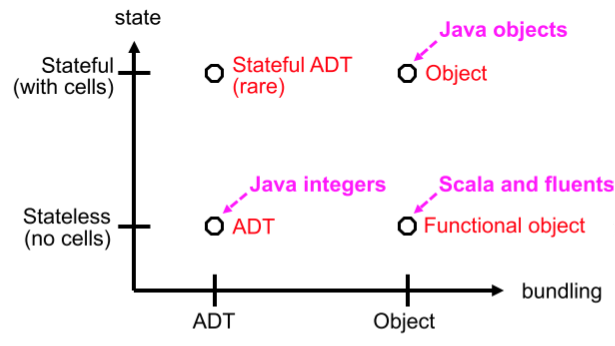
\includegraphics[width=7cm]{img/resAbstract.png}
\caption{Résumé de l'abstraction des données}
\end{figure}

\subsection{Functional Objects}
\subsubsection{Constructions}
Un \textit{objet fonctionnel} n'a pas de sécurité (pas de cellules ni de wrappers) cela utilise que de la programmation \textcolor{red}{d'ordre supérieur}.
\begin{lstlisting}[escapechar=\%]
local 
  fun {StackObject S} 
    fun {Push E} {StackObject E|S} end 
    fun {Pop S1} 
      case S of X|T then S1={StackObject T} X end end 
    fun {IsEmpty} S==nil end
  in
    stack(push:Push pop:Pop isEmpty:IsEmpty) 
  end 
  in 
    fun {NewStack} {StackObject nil} end
end
\end{lstlisting}

\subsubsection{En Scala}
C'est une sorte de forme hybride entre programmation fonctionnel et orienté objet. Scala supporte les 2 \textit{paradigmes}.\\
En Scala, on peut définir des objets immutables qui retournent, \textit{eux-mêmes}, des objets immutables.  Les objets immutables sont des objets \textit{fonctionnels} (\textit{donc pas de changement}).

\subsection{Stateful ADT}
Voici l'implémentation d'un stack en \textit{stateful ADT}:
\begin{lstlisting}[escapechar=\%]
local Wrap Unwrap 
  {NewWrapper Wrap Unwrap} 
  fun {NewStack} {Wrap {NewCell nil}} end 
  proc {Push S E} C={Unwrap S} in C:=E|@C end 
  fun {Pop S} C={Unwrap S} in 
    case @C of X|S1 then C:=S1 X end end 
  fun {IsEmpty S} @{Unwrap S}==nil end
in 
  Stack=stack(new:NewStack push:Push pop:Pop isEmpty:IsEmpty)
end
\end{lstlisting}
On utilise donc à la fois une \textcolor{blue}{cellule} et un \textcolor{blue}{wrapper}. Pour mettre à jour un stack, on n'utilise pas de \textit{wrapper} car on va utiliser des \textit{cellules} (ex: pour \textit{Push, Pop et IsEmpty})

\section{Remarques supplémentaires}
\begin{itemize}
\item Java est fait pour supporter les abstractions de données:
	\begin{enumerate}
	\item True data abstraction (encapsulation, garbage collector)
	\item Tout entité en Java est un \textbf{objet} ou un \textbf{ADT}
	\item Supporte les principes de design orienté objet.
	\end{enumerate}
\item Scala a 2 grands principes:
	\begin{enumerate}
	\item Séparation entre les états mutables et immutables (programmation fonctionnelle)
	\item Tout est un objet (même les fonctions)
	\end{enumerate}
\end{itemize}
Scala, en plus de fonctionner sur la JVM, est un successeur important de Java et est très versatile via sa puissance expressive.

\section{Conclusion}
\noindent
L'abstraction des données est un concept \textcolor{red}{nécessaire} pour construire des programmes plus \textit{complexes}.
\begin{itemize}
\item L'abstraction des données est construite sur: \textit{la programmation d'ordre supérieure, le static scoping, les états explicites, les records et les clés secrètes}
\item L'abstraction des données est définie via ces concepts. Ainsi, on connait la sémantique de l'abstraction de donnée.
\end{itemize} 
Il existe 4 types d'abstraction des données orientées selon 2 axes: 
\begin{enumerate}
\item Objet et ADTs sur un axe
\item Stateful et Stateless
\end{enumerate} 
Il existe 2 types d'abstraction des données qui sont dominantes mais les 2 dernières sont toujours utiles pour certains types d'abstraction.\\
Quasi tous les langages de programmation modernes supportent l'abstraction. Ils supportent généralement \textcolor{blue}{plusieurs} types. Ils sont souvent plus des langages "\textit{orientés abstractions des données}" que simplement "\textit{orienté objet}".


\chapter{Les exceptions}
Une exception est lorsqu'un programme ne se comporte pas comme prévu ou que les inputs ne peuvent pas être utilisé (\textit{par exemple}: division par zéro, fichier non-existant, ...)\\
Ainsi, on peut faire fonctionner le programme même si il rencontre une erreur car celle-ci peut être "\textit{interceptée}" via une \textcolor{blue}{exception}.

\section{Fonctionnement}
On voudrait donc que le programme ne cesse pas quand il rencontre un soucis et on veut qu'une erreur impacte \textit{au minimum} le programme. On utilise le principe du \textcolor{red}{confinement}.

\subsubsection{Le confinement}
\begin{wrapfigure}{r}{.5\textwidth}
\centering
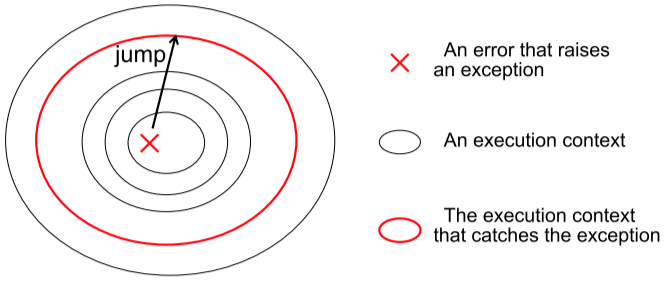
\includegraphics[width=6cm]{img/handler.png}
\end{wrapfigure}
Donc notre programme est un \textcolor{blue}{ensemble imbriqué de contexte d'exécution}.\\
Donc si une erreur apparait, elle influence le contexte et pas tout le programme.\\
On protège chaque exécution par des \textit{exceptions handlers} qui sont comme des "douaniers" entre chaque zone de contexte. Ainsi, on s'assure que l'erreur est contenu et minimisée.

\subsection{En Oz}
On a les \textit{try} et \textit{raise} qui sont deux nouvelles instructions:
\begin{lstlisting}[escapechar=\%]
try <s1> catch <y> then <s2> end	//%On crée l'intercepteur%
raise <x> end											//%On établit une erreur%
\end{lstlisting}

\subsubsection{Try et Raise}
Le \textit{try} met un \textit{marker} sur le stack et puis exécute l'instruction $<S1>$.\\
Si il n'y a aucune erreur, l'instruction s'exécute normalement et le \textit{marker} est enlevé à la fin.\\
Si \textit{raise} est appelé pour signifier une erreur, le stack d'instructions est vidé jusqu'au \textit{marker}. Ensuite, on exécute $<s2>$. Dans notre exemple, $<y>$ est la même erreur que $<x>$. De plus, la porté de <y> couvre exactement jusqu'à $<s2>$.

\subsubsection{Finally}
En plus de ces deux instructions, on peut rajouter une instruction s'appelant \textit{finally} qui comporte des étapes à exécuter peu importe si une erreur arrive ou pas.

\subsection{En Java}
C'est un objet hérité de la classe des \textit{Exceptions} (elle-même sous-classe des \textit{Throwable)} et il existe 2 types d'exceptions:
\begin{itemize}
\item \textcolor{blue}{Checked exceptions}: le compilateur vérifie que les méthodes ne \textit{throw} que des exceptions déclarées pour la classe
\item \textcolor{blue}{Unchecked exceptions}: pour gérer les exceptions que le compilateur ne peut pas vérifier. Elles héritent des \textit{RuntimeException} et \textit{Error}.
\end{itemize}
Donc en tant que développeur on check les erreurs \textit{checked}.

\subsection{Utilisation correcte}
On n'utilise pas une exception pour un comportement \textbf{attendu ou prévisible}. C'est-à-dire que, par exemple, on ne lit pas un fichier jusqu'au moment où il est vide et nous produit une erreur. Non, le fait que le fichier se finisse est prévisible et ne demande pas d'exception.


\chapter{Programmation simultanée}
On a besoin de la \textit{programmation simultanée} car notre monde progresse avec le \textcolor{blue}{temps} et chaque chose progresse indépendamment des autres.
\subsubsection{Simultanéité en programmation}
\noindent
\begin{enumerate}
\item \textcolor{blue}{Système distribué}: relier les pc entre eux par un réseau (data center, ...)
	\begin{enumerate}
	\item Une activité en simultanée est appelée un \textit{noeud de calcul}.
	\item Chaque \textit{noeud de calcul} a ses propres ressources (CPU, mémoire, ...).
	\end{enumerate}
\item \textcolor{blue}{Système d'exploitation}: le controle d'un pc
	\begin{enumerate}
	\item Une activité en simultanée est appelée un \textit{processus}.
	\item Tous les \textit{processus} partagent les mêmes ressources mais ont des espaces allouées de mémoires distincts.
	\end{enumerate}
\item \textcolor{blue}{Processus}: l'exécution d'un seul programme
	\begin{enumerate}
	\item Une activité en simultanée est appelée un \textit{thread}.
	\item Les \textit{threads} partagent le même espace mémoire.
	\end{enumerate}
\end{enumerate}
Ce principe est très naturel car est présent tout autour de nous. Une activité indépendante est donc \textcolor{blue}{simultanée}. Cependant, cela doit être supporté par le langage lui-même.

\section{Les bases}
On peut avoir des événements qui progressent en même temps mais certaines activités doivent pouvoir \textcolor{blue}{communiquer} entre elle et se \textcolor{blue}{synchroniser}.

\subsubsection{Complexité}
On peut faire face à de nombreux soucis en utilisant des \textit{threads}: nondeterminism, race conditions, reentrancy, deadlocks, livelocks, fairness, consistency, shared data.\\

Mais, on peut faire en sorte que la \textit{programmation simultanée} soit aussi simple que la \textcolor{blue}{programmation séquentielle}.\\
Il faut que le paradigme soit correctement choisi. On verra donc le \textcolor{blue}{deterministic dataflow} qui est une forme de programmation fonctionnelle.


\section{Deterministic dataflow}
Les 3 grands paradigmes de la programmation simultanée:
\begin{enumerate}
\item \textcolor{red}{Deterministic dataflow}: (\textit{le plus simple et meilleur})
	\begin{itemize}
	\item Aussi appelé le \textit{functional dataflow}.
	\item Supporte toutes les techniques de la programmation fonctionnelle.
	\end{itemize}

\item \textcolor{red}{Message-passing concurrency}: (Erlang et Scala)
	\begin{itemize}
	\item Les activités envoient des messages entre eux.
	\end{itemize}

\item \textcolor{red}{Shared-state concurrency}: (moniteurs Java)
	\begin{itemize}
	\item Les activités partagent les mêmes données et essayent de travailler ensemble.
	\item Plutôt compliqué et encore fort utilisé aujourd'hui.
	\end{itemize}
\end{enumerate}

\subsubsection{Variable non-liée}
C'est quand on crée une variable dans la mémoire sans qu'elle soit liée à une valeur.\\
En Oz, quand on veut afficher une variable qui n'est pas encore déclarée, Oz va attendre jusqu'à ce qu'on déclare la variable. Donc ci-dessous, Oz va attendre indéfiniment juste avant l'addition de $X$:
\begin{lstlisting}[escapechar=\%]
local X Y in
  Y=X+1
  {Browse Y}
end
\end{lstlisting}
Donc, un Thread peut interagir sur ce code si il attribue une valeur à X. C'est en cela que correspond le \textcolor{blue}{dataflow execution}:
\begin{figure}[H]
\centering
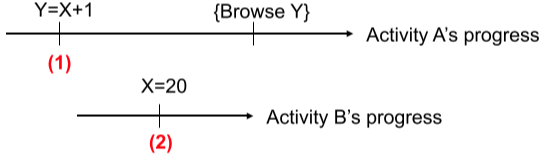
\includegraphics[width=8cm]{img/dataflow.png}
\caption{Exemple d'exécution}
\end{figure}
L'activité A attend à \textcolor{red}{(1)} jusqu'à ce que l'activité B arrive à \textcolor{red}{(2)}.

\section{Threads}
C'est donc cela qui nous permet d'implémenter la programmation simultanée en Oz. C'est donc un \textit{fil} d'exécution qui s'exécute en même temps.\\
Chacun des \textit{Threads} fonctionnent de manière \textcolor{blue}{séquentielle} et sont \textcolor{blue}{indépendants} l'un de l'autre.\\
Cependant il faut bien comprendre quelques détails:
\begin{itemize}
\item Il n'y a aucun ordre spécifique pour l'exécution des Threads.
\item Le système exécute tous les threads en même temps en utilisant l'\textcolor{red}{interleaving semantics}. Donc on a un thread qui exécute un à un les threads et change continuellement.
\item Le système garantit que chaque Thread reçoit les ressources égales et nécessaires.
\end{itemize}
Les Threads peuvent \textit{communiquer} entre eux si ils partagent une variable.\\

\subsubsection{Oz}
En Oz, créer des Threads est très peu "énergivore" donc on peut se permettre d'en créer un grand nombre.\\
De plus, on écrit un Thread comme:
\begin{lstlisting}[escapechar=\%]
thread <s> end
\end{lstlisting}
\noindent
Donc on peut créer ce programme:
\begin{lstlisting}[escapechar=\%]
declare X
thread {Browse X+1} end
thread {X=1} end
\end{lstlisting}
Il y a donc 2 cas de figure possible: ligne 2 $\rightarrow$ ligne 3 ou ligne 3 $\rightarrow$ ligne 2. Cependant, le résultat est le même, 2 est affiché.

\subsubsection{Le Browser}
Le \textit{Browser} en Oz s'exécute avec son propre Thread.\\
Pour chaque variable non-liée qui est affichée, on crée un thread dans le \textit{Browser} qui attend jusqu'à ce qu'on lui attribue une valeur.\\
Cependant, cela ne fonctionne pas avec les \textit{cellules}. Le Browser utilise le paradigme "\textit{functional dataflow}" et il ne regarde donc pas l'intérieur de la cellule.

\subsection{Streams et Agents}
Un stream est une \textcolor{blue}{liste} qui se finit par une variable non défini. On peut étendre la liste autant que l'on veuille. \\
On peut les utiliser comme une façon de communiquer entre des Threads. (ex: \textit{producteur consommateur})

\subsubsection{Producteur Consommateur}
\begin{itemize}
\item \textcolor{red}{Producteur}: génère un stream de données.
\item \textcolor{red}{Consommateur}: lis un stream et réalise une action dessus.
\item \textcolor{red}{Filtre}: lis et génère un stream.
\end{itemize} 

\subsubsection{Agent}
C'est une activité \textit{concurrente} qui lis et écris dans un stream. C'est une raison principale de la \textbf{single assignement} car ainsi on peut faire de la récursion terminale qui fait que le \textit{dataflow deterministic} en un paradigme pratique.\\
Toutes les listes de fonctions peuvent être utilisées comme un agent. (on peut aussi faire la \textit{higher order programming})

\subsection{Sémantique des Threads}
On étend la machine abstraite. Chaque Threads possèdent son propre stack sémantique mais partagent la même mémoire.\\
On exécute une étape du stack sémantique à la fois et à tour de rôle.\\
Le \textcolor{red}{Scheduler} décide quelle thread s'exécute via une technique d'\textit{entrelacement}.

\subsubsection{Entrelacements}
C'est une manière d'aborder des threads plus simples que de la \textit{vraie concurrence}. En entrelacement, les threads d'une processeur ne peuvent pas écrire en même temps sur une zone de mémoire. (on a quand même un \textcolor{blue}{cache coherence protocol} qui s'assure qu'on n'écrit pas en même temps)

\section{Exécution de programmes concurrents}

\subsubsection{Séquentiel}
Une exécution d'un programme séquentiel est son exécution sur un \textcolor{blue}{thread}. Les exécutions séquentielles sont \textcolor{red}{d'ordres totals} donc un \textit{ordre définit entre toutes les pairs d'états}.

\subsubsection{Ordre partiel}
\begin{wrapfigure}{r}{.5\textwidth}
\centering
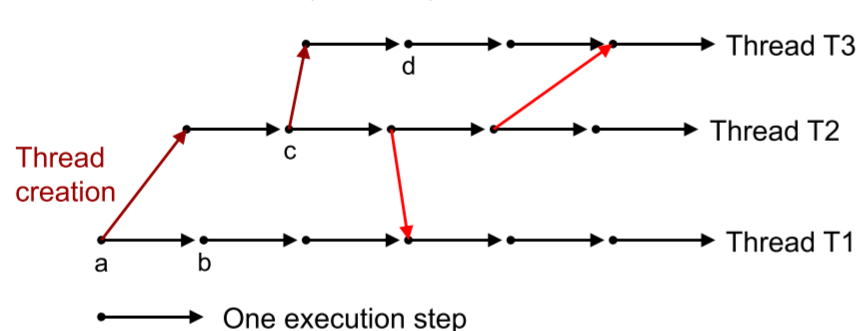
\includegraphics[width=7cm]{img/ordrePartiel.png}
\end{wrapfigure}
Donc un programme concurrent est un programme avec plus qu'un Thread. On dit qu'on a un ordre \textcolor{red}{partiel}. On n'a pas de pair d'exécution définit.\\
Mais on a toujours qu'une seule exécution par étape

\section{Le non-déterminisme}
Le non-déterminisme d'un système est la possibilité d'un système à réaliser des décisions indépendamment de la volonté du développeur.\par
Un exemple typique est le \textcolor{red}{planificateur} (\textit{scheduler}). Il décide quel thread s'exécute à quel moment.\par
Ce principe de non-déterminisme est toujours présent dans un système concurrent. En effet, les activités sont toutes indépendantes et le système doit générer cela de manière non-déterministe.
\subsubsection{Exemple}
On peut penser au fait qu'on ne sait pas qui du thread A ou B s'exécutera en premier. Ce choix varie à l'exécution et est fait par le système.\\
Pareil pour l'écriture dans une cellule qui a un résultat qui varie.\par

\subsubsection{Piège}
\textcolor{red}{Attention}, ce n'est pas parce que 2 threads résultent à un même résultat \textit{tout le temps} qu'ils ne sont pas non-déterministes. Le non-déterminisme est le fait qu'on ne sait pas quel thread se lance en premier.

\subsection{Gestion}
On doit toujours gérer le non-déterminisme et il ne devrait jamais influencer le fait qu'un programme est correct. C'est pour cela qu'on évite d'utiliser des threads \textbf{et} des cellules.

\subsubsection{Deterministic dataflow}
Avec ce paradigme, le résultat d'un programme est toujours le même. Il n'y a aucun non-déterminisme \textcolor{red}{\textit{visible}}.

\subsection{Fonctionnement d'un planificateur}
Le planificateur laisse un thread s'exécuter environ toutes les $10$ ms. On appelle ce temps un \textit{time slice}. (Sur des PC multi-cœurs on peut avoir plusieures exécutions simultanées)\par
Un thread est soit en mode \textcolor{red}{runnable} si l'instruction en haut de son stack \textit{n'attend pas} de variable de \textit{dataflow}. Sinon, il est en état \textcolor{red}{suspended} donc il attend une assignation de variable.

\subsubsection{Équitable}
Un "\textit{scheduler}" est équitable si:
\begin{itemize}
\item N'importe quel thread \textit{runnable} va se lancer dans un temps \textit{fini}.
\item On accorde une priorité à chaque threads mais cela leur accorde juste plus ou moins de pourcentage de \textit{temps} d'exécution.
\end{itemize}
Si un \textit{planificateur} est équitable, on peut s'assurer que notre programme est correct. Sinon, certains programmes ne se lanceraient pas et pourraient produire des réponses erronées.

\section{Concurrency for dummies}
\noindent
\textit{sobrement intitulé par Peter van Roy}\par
En programmation multi-agent, la concurrence n'influence pas le résultat. La concurrence change juste l'ordre d'exécution. On peut ajouter des threads à la volée sans changer le résultat.\par
Cela fonctionne seulement en programmation \textcolor{blue}{fonctionnelle}.\par
Quand on veut \textit{browse} un thread, on aura une sortie sous forme de liste où à la fin on a "$\_$". Cela veut dire qu'on attend une autre information qui pourrait arriver.


\section{Programmation multi-agent}
Par exemple, on fait le crible d'Eratosthène, on va créer une méthode "\textit{producer-consomer}" un peu plus évolué qui relance un thread à chaque exécution. 
\begin{lstlisting}[escapechar=\%]
fun {Sieve Xs}
  case Xs
  of nil then nil
  [] X|Xr then X|{Sieve thread {Filter Xr X} end} 
  end
end 
declare Xs Ys in
thread Xs={Prod 2} end 
thread Ys={Sieve Xs} end
{Browse Ys}
\end{lstlisting}

\section{Digital logic simulation}
Grâce au \textit{deterministic dataflow paradigm} cela est facile à implémenter. Ainsi, on peut implémenter des circuits sans mémoire et avec mémoire qu'on appelle les circuits à logique séquentielle.\par
On représente les \textit{signaux} comme des \textbf{streams} et les \textit{portes logiques} comme des \textbf{agents}.

\subsection{Modélisation}
On sait qu'un signal \textit{digital} est une tension qui évolue en fonction du temps. Les signaux digitaux sont soit $0$ et $1$ mais peuvent avoir du bruits, glitches, résonance, ...\par
Une \textit{porte logique} a une entrée et sortie digitale. Ici, on va simplifier les circuits en supposant qu'ils sont parfaits.

\subsubsection{Signaux comme stream}
On modélise un signal comme un stream avec des $0$ et $1$ tel que $S=a_0 | a_1 | a_2 | ... | a_i | ...$.

\subsubsection{Porte digitale comme agent}
C'est bien plus qu'une fonction booléenne. C'est une \textbf{entité active}. Par exemple:
\begin{lstlisting}[escapechar=\%]
fun {And A B} if A==1 andthen B==1 then 1 else 0 end end 
fun {Loop S1 S2} 
  case S1#S2 of (A|T1)#(B|T2) then {And A B}|{Loop T1 T2} end
end
thread Sc={Loop Sa Sb} end
\end{lstlisting}

\subsubsection{Création multiple}
On va implémenter une \textcolor{red}{abstraction} pour construire plusieurs logic gate. On va nommer cela "\{GateMaker Fun\}". Cela nous crée des gates se basant sur la fonction \textit{Fun}.\par
On a ainsi \textcolor{red}{3} niveaux d'abstraction qu'on peut voir comme de la \textit{programmation orienté objet}.
\begin{enumerate}
\item GateMaker est comme une classe générique, qui fabrique.
\item FunG est comme une classe.
\item La \textit{gate logique} est une sorte d'objet.
\end{enumerate}
\begin{lstlisting}[escapechar=\%]
fun {GateMaker F} 
  fun {$ Xs Ys} 
    fun {GateLoop Xs Ys} 
      case Xs#Ys of (X|Xr)#(Y|Yr) then
        {F X Y}|{GateLoop Xr Yr}
      end 
    end 
  in 
    thread {GateLoop Xs Ys} end 
  end
end
\end{lstlisting}

\subsection{Logique combinatoire}
\begin{wrapfigure}{r}{.5\textwidth}
\centering

\includegraphics[width=5cm]{img/fullAdder.png}
\caption{Un Full Adder}
\end{wrapfigure}
La logique combinatoire \textbf{n'a pas} de mémoire et tous les calculs sont faits en même temps. Donc une gate est une combinaison de fonction et chaque gate peut être inter-connecté.\\
Ceci nous permet d'additionner des nombres et $C_{in}$  permet de prendre en compte une retenu d'un full adder précédent et un $C_{out}$ permet de transmettre une retenu de chiffre.

\subsection{Logique séquentielle}
On a une mémoire des valeurs passées et cela influence. On réalise cela via une gate de délai ou "\textit{Delay gate}". $S=a_0 | a_1 | a_2 | ... | a_i | ...$ et $T=b_0 | b_1 | b_2 | ... | b_i | ...$. On a que $b_i = a_{i-1} \Rightarrow T=0|S$

\subsubsection{Latch}
\begin{figure}[H]
\centering
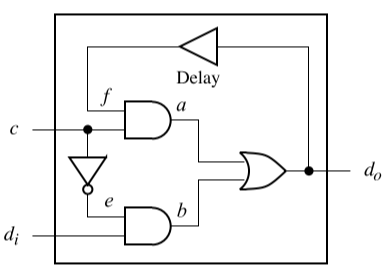
\includegraphics[width=6cm]{img/latch.png}
\end{figure}
Le but est de créer une sorte de bouton pressoir qui une fois pressé reste pressé jusqu'au moment où on represse dessus. Autrement dit, un verrou (\textit{latch}). On peut "\textit{freeze}" le système quand $c = 1$.

\subsection{Résumé}
On construit un programme multi-agent utilisant des streams (liste avec un \textit{tail} non lié) et des agents (des listes fonctionnant sur un thread).\par
On se base sur 2 idées:
\begin{enumerate}
\item \textcolor{blue}{Single-assignement variables} qui synchronise à la liaison
\item \textcolor{blue}{Threads} qui définit une séquence d'instructions exécutés.
\end{enumerate}
Cela n'a pas de déterminisme \textcolor{red}{observable} (pas de "\textit{race conditions}"). Le deterministic dataflow est une forme de programmation fonctionnelle.

\section{Limitations du dataflow deterministique}
Le plus gros soucis est qu'on ne peut pas réaliser des programmes où le \textcolor{red}{non-déterminisme} doit être \textit{visible}. Ceci est important pour les interactions \textit{clients/serveurs}.

\subsection{Client serveur}
On a un ensemble de client communiquant à un serveur. Les clients sont donc des agents \textit{concurrents}. \par 
On peut essayer via un simple code qui prends 2 streams (pour 2 clients) et performe des actions quand on a besoin. \textcolor{red}{Problème} pas \textit{scalable} et quand le client 1 envoie un message cela bloque pour le client 2.\par 
Notre souci est que nous attendons sur des paternes seuls. Avec un \textcolor{blue}{case} on attend sur un seul paterne. Ici, on veut attendre sur de \textbf{multiple} paterne.
\subsubsection{Comprendre le non-déterminisme} 
Le non-déterminisme est un choix fait en dehors du controle du programme. C'est ce qu'on recherche avec le client/serveur car on ne veut pas être retardé car le serveur attend le message d'un autre.

\subsection{Dépasser les limitations}
On va étendre le \textbf{langage kernel} avec nouveau concept. On pourrait faire cela avec une fonction de wait mais cela n'est pas du tout \textit{scalable} car on va devoir attendre et gérer de plus en plus de cas.

\section{Ports}
On va créer des \textcolor{blue}{Ports} qui sont des \textit{streams nommés}. On peut faire:
\begin{lstlisting}[escapechar=\%]
P = {NewPort S} 	// Cree un port P avec son stream S
{Send P X}	 	// Envoie X a la fin du stream du port P
\end{lstlisting}
Ainsi tous les clients envoient leur requête dans ce stream et le serveur se charge de les gérer. Et ainsi cela crée un ordre aléatoire grâce aux \textit{Threads} donc \textit{non-déterministique}.

\subsection{Sémantique}
On a maintenant dans notre langage \textbf{kernel} que $\sigma_1$ stocke les valeurs à assignation unique. $\sigma_2$ stocke les cellules et $\sigma_3$ stocke des ports qui sont des \textbf{paires de variables}.

\subsubsection{Langage kernel}
\begin{lstlisting}[escapechar=\%]
P={NewPort S}, {P %$\rightarrow$%p, S %$\rightarrow$% s} //%$p,s \in \sigma_1$ crée $p=\xi$ et paire $p:s$ à $\sigma_2$%
{Send P S}, {P %$\rightarrow$%p, X %$\rightarrow$% x}	//%$p=\xi$ que $s \in \sigma_1, p:s \in \sigma_2$ crée $s=x|s'$ et update $p:s$%
\end{lstlisting}

L'opération d'ajout à la fin du stream d'un port est \textcolor{red}{atomique} donc cela se fait en \textbf{une seule étape}.

\begin{figure}[H]
\centering
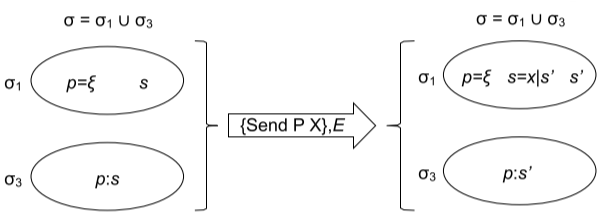
\includegraphics[width=8cm]{img/semantiquePort.png}
\end{figure}

\section{Message-passing concurrency}
C'est un nouveau \textit{paradigme} pour la programmation concurrente. C'est du \textbf{deterministic dataflow} avec des \textbf{ports}. On l'appelle aussi le \textcolor{red}{multi-agent actor programming}.\par 
On a des objets \textit{ports} et des objets \textit{actifs}.

\subsection{Stateless port objects} \label{spo}
Un tel objet est une \textit{combinaison} d'un port, d'un thread et d'une fonction de liste récursive. On appelle aussi cela un \textit{stateless agent}. \par 
Un agent est définit selon sa manière qu'il répond à un message. Chaque agent à son \textbf{propre thread} donc pas de soucis de concurrence.

\subsubsection{Exemple}
On peut définir une fonction simple arithmétique de la sorte:

\begin{lstlisting}[escapechar=\%]
proc {Math M} 
  case M of 
  add(N M A) then A=N+M 
  [] mul(N M A) then A=N*M 
  ... 
  end
end
\end{lstlisting} 
\begin{lstlisting}[escapechar=\%]
MP={NewPort S} 
proc {MathProcess Ms} 
  case Ms of M|Mr then 
    {Math M} {MathProcess Mr}
  end
end

thread {MathProcess S} end
\end{lstlisting}

On peut aussi utiliser un \textcolor{blue}{forAll}

\begin{lstlisting}[escapechar=\%]
proc {ForAll Xs P} 
  case Xs of nil then skip 
  [] X|Xr then {P X} {ForAll Xr P} 
  end
end
\end{lstlisting}
\begin{lstlisting}[escapechar=\%]
proc {MathProcess Ms} 
  {ForAll Ms Math} 
end
\end{lstlisting}


Pour construire des objets ports stateless de manière générique. Notre deuxième implémentation utilise la syntaxe des \textit{for loops}. 
\begin{lstlisting}[escapechar=\%]
fun {NewPortObject0 Process} Port Stream in
  Port={NewPort Stream} 
  thread {ForAll Stream Process} end 
  Port
end
\end{lstlisting}
\begin{lstlisting}[escapechar=\%]
fun {NewPortObject0 Process} Port Stream in
  Port={NewPort Stream} 
  thread for M in Stream do {Process M} end end 
  Port
end
\end{lstlisting}

\subsection{Stateful port objects}
\begin{wrapfigure}{r}{.4\textwidth}
\centering
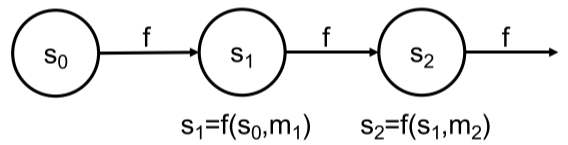
\includegraphics[width=6cm]{img/statefulPortObject.png}
\end{wrapfigure}
C'est donc la même chose qu'au \ref{spo} mais ici, les agents ont une \textbf{mémoire}.\par 
On appelle sa \textit{mémoire interne} un "\textcolor{blue}{state}" qui est défini comme ci-contre.\par 
On a des fonctions de \textit{transition} qui passe d'état en état. Cette fonction est de type $F	: State \times Msg \longrightarrow State$.
\begin{lstlisting}[escapechar=\%]
fun {NewPortObject Init F} 
  proc {Loop S State} 
    case S of M|T then 
      {Loop T {F State M}} end
  end 
    P
in
  thread S in P={NewPort S} {Loop S Init} end 
  P
end
\end{lstlisting}
\begin{lstlisting}[escapechar=\%]
proc {Loop S State} 
  case S of M|T then {Loop T {F State M}} end
end
\end{lstlisting}
La fonction $F$ dans notre \textit{loop} est une fonction binaire qui part d'un état initial et effectue différentes opérations. Ce n'est rien d'autre qu'un \textit{Fold}.

\subsection{Exemples}
\subsubsection{Updated NewPortObject}
\begin{lstlisting}[escapechar=\%]
fun {NewPortObject Init F} 
  P Out
in
  thread S in P={NewPort S} Out={FoldL S F Init} end 
  P
end
\end{lstlisting}
$Out$ est l'état final qui termine les agents.

\subsubsection{Cell Agent}
\begin{lstlisting}[escapechar=\%]
fun {CellProcess S M} 
  case M 
  of assign(New) then New 
  [] access(Old) then Old=S S 
  end
end
\end{lstlisting}
Notre agent se comporte comme une \textit{cellule}. Les cellules et les ports sont équivalents en terme d'expression.

\subsubsection{Uniform Interface}
\begin{lstlisting}[escapechar=\%]
// %On crée et utilise un \textit{cell agent}%
declare Cell 
Cell={NewPortObject CellProcess 0} 
{Send Cell assign(1)}
local X in {Send Cell access(X)} {Browse X} end

// %On veut avoir les mêmes interfaces en tant qu'objet%
{Cell assign(1)} 
local X in {Cell access(X)} {Browse X} end

// %On change la sortie pour être une procédure%
fun {NewPortObject Init F} 
  P Out
in
  thread S in P={NewPort S} Out={FoldL S F Init} end 
  proc {$ M} {Send P M} end
end
\end{lstlisting}

\section{Active objects}
C'est un object qui est une sorte de "\textit{port object}" et qui a des comportements comme une classe. Donc on a le \textit{polymorphisme} et l'\textit{héritance} de classe tout en ayant du "\textit{message passing}".

\subsection{Définition Classe et Objet}
\begin{lstlisting}[escapechar=\%]
class Counter 
  attr i 
  meth init(X) 
    i := X
  end 
  meth inc(X) 
    i := @i + X
  end 
  meth get(X) 
    X=@i
  end
end
\end{lstlisting}
\begin{lstlisting}[escapechar=\%]
{Ctr inc(10)} 
{Ctr inc(5)} 
local X in 
  {Ctr get(X)} 
  {Browse X}
end
\end{lstlisting}
Pour initialiser un objet, on réalise l'opération $CTR=$ \textit{\{New Counter init(0)\}}.

\subsubsection{Active Object}
\begin{lstlisting}[escapechar=\%]
fun {NewActive Class Init} 
  Obj={New Class Init} 
  P
in
  thread S in 
    {NewPort S P} 
    for M in S do {Obj M} end
end 
  proc {$ M} {Send P M} end
end
\end{lstlisting}
On combine donc les classes et les ports mais on utilise l'interface \textit{uniforme} de Oz pour leur donner l'apparence d'un objet standard en Oz.

\subsection{Différence entre passif et actif}
On appelle passif, les objets en Oz qui ne s'exécute \textbf{pas dans leur propre thread}. Les actifs eux ont leur propre thread d'exécution.

\subsubsection{Avantage}
On peut sans aucun risque appeler un objet actif car ses données sont dans son propre thread à l'inverse des passifs. \par 
Dans un objet passif, ses méthodes peuvent s'exécuter de manière \textbf{concurrente} à l'inverse des actifs qui seront toujours \textbf{séquentielle}.\par 
Les objets passifs ne sont pas \textit{concurrency-safe}.

\newpage
\section{Message protocol}
\begin{wrapfigure}{r}{.5\textwidth}
\centering
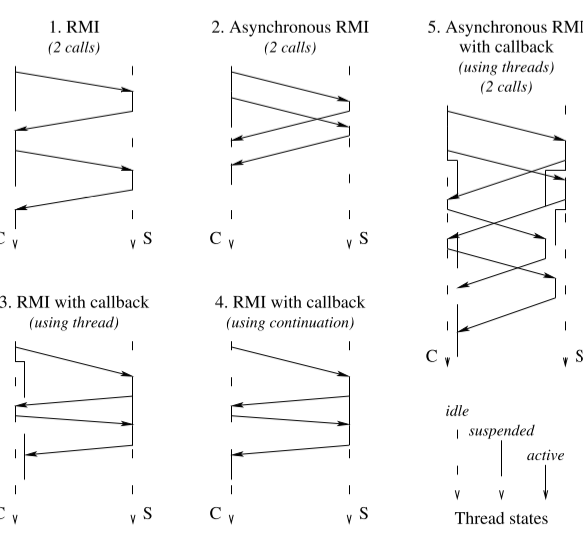
\includegraphics[width=6cm]{img/message.png}
\end{wrapfigure}
Ce sont des \textit{séquences} de messages entre plusieurs parties qui peuvent être comprises à des niveaux d'abstractions plus élevés que les messages \textit{individuels}.\par 
On commence avec un RMI simple et puis on fait des appelles asynchrones et on y en rajoute. \par 
Le protocole le plus compliqué est le \textbf{RMI asynchrone avec callbacks}.\par
En gros, \textbf{RMI} c'est le fait d'envoyer des messages et recevoir des messages. \textbf{Asynchrone}, on n'attend pas le message de retour d'un serveur. \textbf{Callback}, on envoie un message à un serveur et on lui envoie un port où il peut envoyer son message.

\section{Memory Management \& Garbage Collection}

Si jamais on réalise un programme qui boucle et possède une variable qu'on incrémente à chaque fois, on va se retrouver avec $n$ variables alors que nous n'avons besoin que d'une seule.\par 
Notre stack d'instruction est constant via la \textcolor{red}{last call optimization} mais notre mémoire ne fait que grandir.

\subsection{La représentation des données dans la mémoire}
On utilise des \textit{memory words} qui prennent \textit{64-bit}. Au démarrage d'un programme, le système attribue un certain nombre de \textit{memory words} pour son exécution. Ce nombre peut varier et est géré par le programme.

\subsubsection{Cycle de vie des mots}
Il y a \textbf{3 états} distincts: \textit{actif}, \textit{inactif} et \textit{libre}. Au début, tout est libre. Un mot devient actif quand il est \textit{alloué} et devient inactif si on ne l'utilise plus. Un mot redevient libre si on le \textit{libère} quand il est actif ou s'il est manuellement ou automatiquement (\textit{garbage collector}) retourné en mode libre depuis l'état inactif.\par 
Bien évidemment on voudrait qu'un mot plus utilisé et inactif redevienne libre pour qu'il puisse libérer de la place.

\subsubsection{Soucis}
Quand on veut rappeler des mots supposés \textit{inactifs}, on peut avoir du \textcolor{red}{dangling reference}. C'est quand on veut reprendre un mot mais qu'il va être utilisé par le programme (\textit{segfault}). On a aussi des \textcolor{red}{memory leak} où des mots ne sont jamais rappelés et causent des ralentissements et des utilisations de la mémoire inutile.

\subsubsection{Inactif}
Un mot est considéré comme \textbf{inactif} quand on peut plus y accéder depuis le stack.\\
L'exécution d'un programme est déterminé par le \textit{stack}. Il faut bien s'assurer qu'il n'existe plus de chemin indirect menant à une variable avant de la considérer comme inactive.

\subsubsection{Rappel}
On peut soit le faire manuellement (avec des free et malloc en \textit{C}) mais pas facile. Ou bien, on utilise un \textit{garbage collector} (ramasse-miette) qui est plus pratique et robuste si bien implémenté.

\subsection{Active memory versus memory consumption}
\begin{itemize}
\item \underline{La mémoire active:} combien de mots le programme a besoin à un certain temps. Une \textbf{in-memory database} a une grande quantité de mémoire active mais une petite consommation (car on n'utilise qu'une partie de la database).
\item \underline{La consommation de la mémoire:} est la quantité de mots alloués par unité de temps. Donc une \textbf{simulation du mouvement des molécules dans une boite} a une grand consommation de mémoire mais peu de mémoire active.
\end{itemize}

\section{Deterministic dataflow with ports}
Simplifie l'utilisation de programme concurrent. On y ajoute des ports si nécessaire.

\subsection{Composition concurrente (nombre fixe de Thread)}
Cela permet de la composition concurrente (dynamique ou statique) et élimine les dépendances séquentiels.\\
Si on a plusieurs thread, parfois on doit revenir au principal. Donc le thread original attend que les autres s'arrêtent. C'est ce qu'on appelle la composition concurrente.
\begin{lstlisting}[escapechar=\%]
%$(<s>_1 \parallel <s>_2)$%  	 // %Crée deux threads et attend que les deux se terminent%
%$<s>_3$%		// %S'exécute que quand les deux se terminent%
\end{lstlisting}

\subsubsection{Implémentation}
\begin{lstlisting}[escapechar=\%]
local X1 X2 in
  thread %$<s>_1$% X1 = unit end
  thread %$<s>_2$% X2 = unit end
  {Wait X1}
  {Wait X2}
 end
\end{lstlisting}
On implémente cela en utilisant des variables \textit{dataflow}. On va utiliser la constante \textcolor{blue}{unit} quand la valeur n'importe pas.\par 
L'ordre dans lequel on attend n'influence pas le résultat.

\subsubsection{Higher-order abstraction}
On va définir une fonction \textit{\{Barrier Ps\}} avec une liste d'instruction $Ps$.
\begin{lstlisting}[escapechar=\%]
proc {Barrier Ps} 
  Xs={Map Ps fun {$ P} X in thread {P} X=unit end X end}
in 
  for X in Xs do 
    {Wait X} 
  end
end
\end{lstlisting}
Cette fonction \textit{Barrier} peut être réalisée grâce au \textit{deterministic dataflow} uniquement.\par 
Donc on peut créer une abstraction pour cela de type: $\textcolor{blue}{conc} <s>_1 \parallel <s>_2 \parallel ... \parallel <s>_n \textcolor{blue}{end}$ qui la même chose que $\{Barrier [\textcolor{blue}{proc} \{\$\} <s>_1 \textcolor{blue}{end} \quad \textcolor{blue}{proc} \{\$\} <s>_2 \textcolor{blue}{end} \quad ... \quad \textcolor{blue}{proc} \{\$\} <s>_n \textcolor{blue}{end} ]\}$

\subsection{Composition concurrente (nombre variable de Thread)}
On doit arriver à créer de nouveaux threads qui se synchronisent avec les threads actuels. Cette abstraction \textcolor{red}{ne peut pas} être écrite en deterministic dataflow. Effectivement, l'ordre de création est inconnu donc \textbf{non-déterministique}. On va définir cela avec un port.

\subsubsection{Spécification de l'abstraction}
Le Thread principal attend que les autres se terminent. 
\begin{lstlisting}[escapechar=\%]
{NewThread proc {$} <s> end SubThread} 
{SubThread proc {$} <s> end}
\end{lstlisting}
\begin{wrapfigure}{r}{.5\textwidth}
\centering
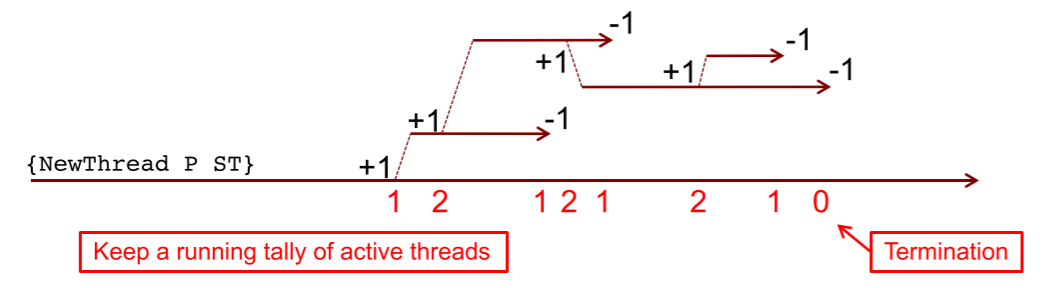
\includegraphics[width=8cm]{img/newThread.png}
\end{wrapfigure}
La fonction \textit{NewThread} crée un nouveau calcul $<s>$ dans le thread \textit{principal} et ressort dans la procédure \textit{SubThread}.\par 
Donc le \textit{NewThread} se termine qu'après que tous les \textit{SubThread} se terminent. \textit{SubThread} crée un second thread avec $<s>$. Les deux $<s>$ peuvent appeler le \textit{SubThread} et ainsi de suite récursivement. On a ainsi une profondeur d'arbre arbitraire.\par 
On utilise un \textbf{port} pour compter le nombre de \textit{Threads} actifs. 
\begin{lstlisting}[escapechar=\%]
proc {NewThread P SubThread} //SubThread is an output 
  S Pt={NewPort S}
in
  proc {SubThread P} 
    {Send Pt 1} 
    thread 
      {P} {Send Pt ~1} //Minus sign is tilde
    end
  end 
  {SubThread P} //Main computation 
  {ZeroExit 0 S} //Keep running sum on S and stop when 0
end
\end{lstlisting}
Pour que cela soit correct, on doit bien incrémenter avant de créer un thread et dé-incrémenter juste avant de le finir sinon on pourrait parfois tomber à 0 threads actifs en cours d'exécution alors que ce n'est pas vraiment le cas.
\subsubsection{Usage de l'invariant}
On pose que la somme des éléments $S$ doit être supérieur ou égal au nombre de threads actifs. Si on tombe à $0$ on a donc tout fini.\par 
On a 4 actions à une exécution:
\begin{enumerate}
\item On envoie 1: donc notre invariant est vrai
\item On commence un thread: cela se base sur la véracité du premier point. Cela est donc vrai aussi.
\item On retire 1: le thread ne fait plus rien d'utile et on le fait juste avant de le supprimer. Donc toujours vrai.
\item On arrête le Thread: rien de spécial, toujours vrai.
\end{enumerate}
On va créer une procédure \textit{\{ZeroExit N S\}} qui voit si on tombe à 0:
\begin{lstlisting}[escapechar=\%]
proc {ZeroExit N S}
  case S of X|S2 then
    if N+X==0 then skip 
    else {ZeroExit N+X S2} end
  end
end
\end{lstlisting}

\subsection{Conclusion}
3 grands paradigmes pour la programmation concurrente:
\begin{enumerate}
\item \textcolor{red}{Deterministic Dataflow}: le meilleur mais ne peut pas exprimer le \textit{non-déterminisme} ( qui est utile dans le cloud).
\item \textcolor{red}{Message Passing}: très général mais plus compliqué. On a des "\textit{stateful agents}" qui communiquent entre eux avec des messages \textbf{asynchrones}. (Erlang)
\item \textcolor{red}{Deterministic Dataflow with Ports}: meilleur approche. On écrit un programme en grande partie comme en \textit{deterministic dataflow}. On y ajoute des ports quand on en a besoin.
\end{enumerate}

\chapter{Erlang}
\section{Introduction}

\subsection{Force d'Erlang}
On a des agents (processus) qui sont légers et s'envoient des \textbf{messages} entre eux. Via cela, on peut avoir de la concurrence et avoir de nombreux processus qui fonctionnent ensemble et parallèlement. On peut ainsi faire des programmes sur plusieurs pc. Il y a une vision de "\textit{Let it fail}" car le langage est robuste et sait intercepter et traiter des erreurs. Si une composante ne fonctionne pas, tout le programme ne s'arrête pas nécessairement. On a des arbres \textbf{superviseurs} qui regardent s'il y a des erreurs.

\subsection{Les bases}
Erlang est composé de processus qui sont des "\textit{active agents}" qui communiquent de manière asynchrone via du "\textcolor{red}{asynchronous FIFO message passing}". Erlang ne partage rien, toutes les données sont copiées. En erlang, chaque processus a une sorte de boite au lettre qui est accessible via \textbf{pattern matching} et ne dépend pas de l'ordre.

\section{Les performances}
Pour créer de nouveaux processus et pour envoyer des messages entre, Erlang est extrêmement rapide. Cela est très utile pour des sites web. Là où Apache crash à 4000 requêtes simultanées et une bande passante qui se dégrade, Erlang peut en avoir 40000.
\subsection{Switch AXD301}
C'est un switch pour la télécommunication qui est basé sur Erlang et agrémenté via du Java et C. On a une perte linéaire quand on a une surcharge. Quand on demande $1000\%$ des capacités du switch, on a $40\%$ d'efficacité. AXD 301 version 3.2 a 1MLOC Erlang, 900KLOC C/C++, 13KLOC Java.

\section{Concept de Base}
\subsection{Pure Fonctional Core}
Dans chaque processus, Erlang fonctionne comme un langage purement fonctionnel. Chaque variable à une assignation unique. Les fonctions sont des valeurs avec du "\textit{lexically scoped higher-order programming}". Le pattern matching est utilisable dans les \textit{case}, \textit{if} et \textit{receive}.\par 
Toutes les données sont symboliques. Les types de données sont similaires à Oz mais on a également les \textcolor{red}{binary vectors} (utilisé pour les calculs de protocoles). 

\subsection{Organisation}
Un programme en Erlang est composé de \textit{module} dont chaque fichier s'écrit comme suit: (ex: dans un fichier \textit{math.erl})
\begin{lstlisting}[escapechar=\%, language=erlang]
-module(math).
-export([areas/1]).
-import(lists, [map/2]). 

areas(L) -> lists:sum(map(fun(I) -> area(I) end, L)).

area({square,X}) -> X*X;
area({rectangle,X,Y}) -> X*Y.
\end{lstlisting}
L'export montre les fonctions à exporter et on y indique le nombre d'arguments. On importe des modules et fonctions. On a ainsi une dépendance de modules.

\section{Message Passing}
\subsection{Création et envoi}
On va créer un nouveau processus qui exécute la fonction "\textit{Fun}" via la fonction "\textit{spawn}". \textcolor{red}{Pid = spawn(Fun)}. Cela nous renvoie un identifiant de processus. La fonction "\textit{Fun}" peut être anonyme ou non. Le Pid est unique et constant. \par 
On envoie un message via \textcolor{red}{Pid ! Message}. Cela s'envoie de manière asynchrone et toutes les données sont copiées.

\subsection{Réception}
On intercepte un message via un \textcolor{blue}{receive}. La boite au lettre est une liste trié de message. On les récupère via le receive puis on fait du pattern matching.\\
Si la boite au lettre est vide, le processus attend. Sinon, il essaye de match avec un des cas possibles et l'exécute. Si rien ne match, alors le receive se bloque et attend le prochain message. Le message reste dans la boite au lettre dans ce cas. Il faut éviter que cela reste indéfiniment dans la boite au lettre sinon \textit{memory leak}. \par
Patterns est une structure de donnée symbolique contenant des identificateurs de variable et des gardes qui sont de simples tests.

\section{Process Linking}
On relie \textcolor{blue}{Pid1} à \textcolor{red}{Pid2}. Pid1 appelle \textbf{link(\textcolor{red}{Pid2})} pour faire une liaison. Et vice versa pour en faire une bidirectionnelle.

\subsection{Exit}
Un processus s'arrête et envoie un \textbf{signal d'exit}. Il envoie la raison de son arrêt aux processus qui sont reliés. Si le processus s'arrête normalement, il renvoie l'atome "\textit{normal}". Si il rencontre une erreur à l'exécution il renvoie quelque chose comme \textcolor{red}{\{Reason, Stack\}}. Le comportement classique est que tous les processus s'arrêtent à cause de l'erreur. On peut aussi capturer des erreurs via "\textit{process\_flag(trap\_exit, true)}". Ainsi, cela est envoyé comme un message sous forme \textcolor{red}{\{‘EXIT’, FromPid, Reason\}}. On peut également tuer un processus via la fonction exit.

\section{Changement dynamique}
On peut, en Erlang, modifier le code qui est en cours d'exécution. On a ainsi \textcolor{red}{2} versions des modules qui sont présentes. Les processus peuvent choisir de continuer avec l'ancien processus ou le nouveau. Si on utilise \textcolor{red}{m:Fun} cela force à utiliser la nouvelle version. 

\section{Abstraction pour des programmes robustes}
Les erreurs ne peuvent être évitées et donc on les manipule. Les fonctions sont \textcolor{red}{fail-fast} pour éviter les problèmes. Les erreurs sont détectables et les programmes ne partagent pas d'états entre eux.

\subsection{Slogan}
\begin{itemize}
\item \textbf{Let it fail}: On ne peut pas toujours éviter les erreurs et on doit faire avec. On simplifie les erreurs et on s'y attend.
\item \textbf{Let some other process do error recovery}: On va utiliser des processus superviseur pour s'occuper des erreurs et relancer le programme. 
\item \textbf{Do not program defensively}: On ne fait pas de "check" d'erreur. Cela n'enlève pas toutes les erreurs et alourdit le programme sinon (fail-safe).
\end{itemize}

\subsection{Erlang et OTP système}

\subsubsection{Systèmes}
On a une certaine hiérarchie dans les \textbf{systèmes}:
\begin{enumerate}
\item \textcolor{red}{Release}: Contient toutes les informations pour construire et exécuter un système.
\item \textcolor{red}{Application}: Contient tout le logiciel nécessaire pour faire fonctionner une application. Souvent indépendantes l'un de l'autre et avec une certaine hiérarchie.
\item \textcolor{red}{Behavior}: Un ensemble de processus qui ensemble implémente un pattern concurrent. Donc contient un superviseur.
\item \textcolor{red}{Worker}: Un processus qui est une instance d'un comportement. (typiquement: \textit{gen\_server, gen\_event ou gen\_fsm})
\end{enumerate}

\subsubsection{Comportement}
On a 5 comportements:
\begin{enumerate}
\item \textcolor{red}{Generic server (gen\_server)}: pour construire une architecture client/serveur. On a des registres, timeout, start/stop, state management, appel (a)synchrone, erreur.
\item \textcolor{red}{Generic event handler/manager (get\_event)}: event handlers comme des logs qui répondent à des streams d'évènements et envoie et reçoit des notifications.
\item \textcolor{red}{Generic finite state machine (gen\_fsm)}: Applications (ex: protocol stack) peuvent être représenter comme des machines d'états finis. On a un ensemble d'état et d'évènement qui donnent des actions et états.
\item \textcolor{red}{Application}: composant qui peut être initié et arrêté. Il est réutilisable.
\item \textcolor{red}{Supervisor}: arbre superviseur.
\end{enumerate}
Ces comportements caches la plupart de la complexité de chaque concept. Surtout pour la concurrence et la tolérance à l'erreur.

\section{arbre superviseur}
Les arbres superviseurs prennent l'avantage que des erreurs sont souvent temporaires, donc si on échoue, on relance le processus.

\subsection{Structure et principe}
\begin{wrapfigure}{r}{.5\textwidth}
\centering
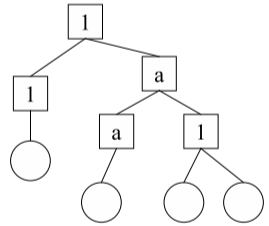
\includegraphics[width=6cm]{img/hierarchies.png}
\end{wrapfigure}
On a donc un arbre où la root est le noeud qui supervise ses branches. Elle arrête et relance des nodes enfants. Les superviseurs sont eux-mêmes inspectés pour éviter qu'ils crashent. On les démarre via un processus synchrone afin que l'état initial soit correct.\\
On a différente méthode de redémarrage comme: \textcolor{red}{one\_for\_one \textbf{1} (redémarre un seul), one\_for\_all \textbf{a} (redémarre tous les enfants), rest\_for\_one}. On est limité par le nombre de restart possible par interval. Si on excède cela, un superviseur plus élevé prend le relais. Cela est construit ainsi pour éviter les crash en continu.\\
Les $\square$ représente des superviseurs et les travailleurs sont représentés via $\bigcirc$.

\section{Conclusions}
La plateforme \textcolor{red}{Erlang/OTP} est une combinaison de Erlang et de librairie standard OTP qui permet de construire des programmes robustes et des systèmes distribuées:
\begin{itemize}
\item Erlang: processus (agent actif) qui s'envoie des messages asynchrones et ne partagent pas d'état.
	\begin{itemize}
	\item Tous les processus sont définis en programmation fonctionnelle et supporte des mises à jour dynamiques.
	\item On détecte les erreurs (fait partie du \textit{process linking}).
	\end{itemize}
\item OTP: permet d'avoir des programmes robustes en utilisant les comportements, test et arbres superviseurs.
	\begin{itemize}
	\item Un comportement est un pattern générique de concurrence. 
	\item Un arbre superviseur contrôle comment gérer les erreurs.
	\item Les tests sont faits pour la concurrence et les systèmes distribués. On peut y injecter des erreurs.
	\end{itemize}
\end{itemize}



\chapter{Conseils pour la syntaxe d'Oz}
Voici une liste d'astuces et de choses importantes à savoir sur Oz:
\begin{itemize}
\item Déclarer vos fonctions et variables avec une \textbf{majuscule} au début!
\item Une procédure est une fonction qui ne retourne \textbf{rien}.
\item Pour retourner une valeur dans une fonction, on écrit une ligne où on ne fait \textit{aucune} assignation ou opération, ... (Ex: on veut retourner $X$ on écrit sur une ligne $X$ tout seul)
\item Pour éviter d'avoir des surprises, toujours bien terminer sa liste par un $| nil$
\item On peut toujours utiliser une fonction récursive avec \textbf{accumulateur} pour une fonction récursive. C'est même conseillé !
\item On peut écrire en langage Kernel directement en oz
\item On peut faire des listes de procédures via la notation Kernel d'une procédure
\item Une liste est un tuple de type (1:Num 2:(1:Num 2:nil))
\item Pour être plus "opti" utiliser les local in.
\item Si notre code est le même que celui du voisin mais que vous avez des résultats différents, \textit{relancez emacs ou VScode}. Nettoyer le buffer et feed tout le code dedans.
\item Pour être plus \textit{productif}, télécharger "Powertoys" sur Windows et activer l'option "\textbf{toujours afficher}" (\textbf{always on top}).
\end{itemize}


\end{document}


